% acoustic_modem_algorithms.tex
% Algorithms of the acoustic modem demo, version 3 (acoustic_modem_v3.html, audiocomm_v3.py), version 2 (acoustic_modem_v2.html = acoustic_modem.html, audiocomm_v2.py) and version 1 (acoustic_modem_v1.html, audiocomm_v1.py).
% Compile with: pdflatex acoustic_modem_algorithms.tex (twice, for the references and the table of contents).
\documentclass[11pt,a4paper]{article}
\usepackage[T1]{fontenc}
\usepackage[utf8]{inputenc}
\usepackage{lmodern}
\usepackage{microtype}
\usepackage[margin=2.4cm]{geometry}
\usepackage{amsmath,amssymb,amsthm,mathtools,bm}
\usepackage{booktabs,tabularx,array}
\usepackage{enumitem}
\usepackage{caption}
\usepackage{float}
\usepackage{xcolor}
\usepackage{tikz}
\usetikzlibrary{arrows.meta,positioning,decorations.pathreplacing,calc,fit}
\definecolor{icemagenta}{HTML}{86144F}
\definecolor{iceink}{HTML}{1C1722}
\definecolor{icegrey}{HTML}{706A7F}
\definecolor{iceground}{HTML}{F5F3F6}
\usepackage[colorlinks=true,linkcolor=icemagenta,citecolor=icemagenta,urlcolor=icemagenta]{hyperref}
\usepackage[nameinlink,capitalise,noabbrev]{cleveref}

\newcommand{\kHz}{\,\mathrm{kHz}}
\newcommand{\Hz}{\,\mathrm{Hz}}
\newcommand{\ms}{\,\mathrm{ms}}
\newcommand{\dB}{\,\mathrm{dB}}
\newcommand{\E}{\mathbb{E}}
\newcommand{\round}[1]{\operatorname{round}\!\left(#1\right)}
\newcommand{\clip}{\operatorname{clip}}
\newcommand{\maxstar}{\operatorname{max}^{*}}
\newcommand{\code}[1]{\texttt{#1}}
\newcommand{\fsT}{f_{\mathrm{s}}^{\mathrm{T}}}
\newcommand{\fs}{f_{\mathrm{s}}}
\newcommand{\Rc}{R_{\mathrm{c}}}
\newcommand{\NP}{N_{\mathrm{P}}}
\newcommand{\NH}{N_{\mathrm{H}}}
\newcommand{\nc}{n_{\mathrm{c}}}
\newcommand{\nz}{n_{0}}

\theoremstyle{remark}
\newtheorem*{remark}{Remark}

\setlist{itemsep=2pt,topsep=4pt}
\setlength{\emergencystretch}{2em}
\renewcommand{\arraystretch}{1.15}
\captionsetup{font=small,labelfont=bf}

\title{\color{icemagenta}\textbf{An acoustic modem for the classroom}\\[4pt]
\large Algorithms, equations and parameter choices of the demo, version~3}
\author{Communication Theory (2A), CentraleSup\'elec\,---\,Mention ICE}
\date{9 October 2026\\[2pt]\small Describes \code{acoustic\_modem\_v3.html} and \code{audiocomm\_v3.py}; version~2, \code{acoustic\_modem\_v2.html}\\ (also served as \code{acoustic\_modem.html}) and \code{audiocomm\_v2.py}; and version~1, \code{acoustic\_modem\_v1.html} and \code{audiocomm\_v1.py}}

\begin{document}
\maketitle

\begin{abstract}
\noindent
The demo sends text, images and room soundings from a laptop's speaker to the students' phones through the air of the classroom.
This document describes every algorithm the modem implements, with the equations behind them, and explains the values chosen for its parameters.
The transmitter uses frequency-shift keying (FSK) with two tones per symbol or, since version~2, four tones carrying two bits, either on fixed tones or hopping over up to 32 tone pairs or 16 groups of four tones; at 6400 bit/s, one group of four tones covers the whole band.
Version~3 adds orthogonal frequency-division multiplexing (OFDM): 546 or 273 subcarriers carrying differential QPSK, with a guard interval of 21 or $5\ms$, at 17 or 20\,kbit/s before the code.
Each frame is self-describing: a control part that every receiver knows in advance carries a maximum-length-sequence preamble and a protected header, so receivers need no settings.
Four error-correcting codes can be sent: none, Hamming $(7,4)$, the $K=7$ convolutional code, and a turbo code of rate $1/2$, $1/3$ or $1/4$.
Reed--Solomon $(255,223)$ is received but no longer sent.
The FSK receiver is non-coherent.
It detects the frame by correlating a level-free tone contrast with the preamble, tracks the symbol timing with an early--late gate, and estimates the clock offset between the two devices from a postamble.
It turns the tone energies into log-likelihood ratios (LLRs) with a Rician model calibrated on known bits, then decodes with soft-decision Viterbi or iterative log-MAP decoding.
A room-sounding frame measures the impulse response of the speaker, room and microphone with a periodic maximum-length sequence, and derives the reverberation time, the direct-to-reverberant ratio, $C_{50}$, the delay spread, the frequency response and the signal-to-noise ratio per frequency.
Numbers quoted as results come from the simulations and the one real recording documented in \code{audioComm\_two\_devices.md}.
Version~2 differs from version~1 by the four-tone mode (\cref{sec:mfsk}) and a narrower search for the postamble (\cref{sec:clock}); the text says where.
Version~3 adds OFDM (\cref{sec:ofdm}), received by differential detection after a timing and a time-scale estimate on two reference symbols.
\end{abstract}

\tableofcontents
\newpage

%======================================================================
\section{Overview}
\label{sec:overview}

\subsection{Files and scope}
\begin{itemize}
\item \code{acoustic\_modem\_v3.html} and \code{audiocomm\_v3.py} are version~3: version~2 plus OFDM as a third modulation (\cref{sec:ofdm}). They send the same FSK frames and room soundings as version~2, bit for bit, and read all of version~2's frames; earlier pages and scripts ignore OFDM frames.
\item \code{acoustic\_modem\_v2.html} is the web page of version~2: transmitter and receiver in one self-contained file, with no network access needed once loaded. The modem core is plain JavaScript, independent of the page's user interface. \code{acoustic\_modem\_v1.html} is version~1, and \code{acoustic\_modem.html} is a copy of the version that the GitHub Pages address serves, now version~2.
\item \code{audiocomm\_v2.py} (numpy only) implements the same transmitter bit for bit and the same receiver in vectorised form, together with the room simulator of \cref{sec:roomsim}; \code{audiocomm\_v1.py} is its version~1. Their few differences from the page's receiver are listed in \cref{sec:pydiff}.
\item The page and the script of a version produce byte-identical WAV files and decode each other's recordings. Version~1 also reads every version~0 frame. Version~2 is version~1 plus four-tone FSK (\cref{sec:mfsk}) and a narrower search for the postamble (\cref{sec:clock}): it sends the same binary frames as version~1 and reads all of version~1's frames, while versions~0 and~1 ignore its four-tone frames. Version~0 (\code{acoustic\_modem\_v0.html}, \code{audiocomm.py}) is frozen and is the subset of version~1 without tone hopping, the turbo code and room sounding. The MATLAB scripts use an older frame and are not described here.
\end{itemize}

\subsection{Signal chain}
\Cref{fig:chain} shows the processing chain.
The transmitter builds a frame of bits (\cref{sec:frame}), maps each bit to a tone burst (\cref{sec:mod,sec:hop}), and plays it at $\fsT = 48\kHz$.
The receiver records at its own rate $\fs$ (usually $44.1$ or $48\kHz$), with echo cancellation, noise suppression and automatic gain control switched off, and runs the steps of \cref{sec:rx}.

\begin{figure}[ht]
\centering
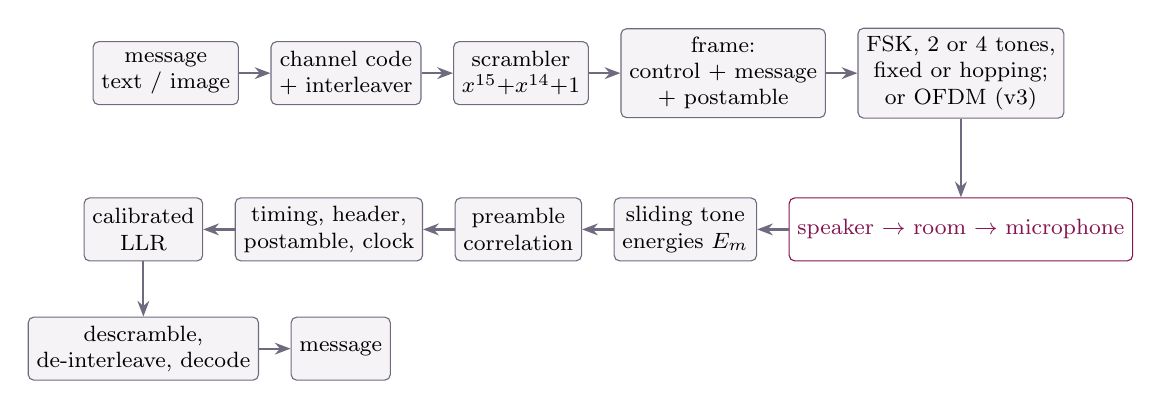
\begin{tikzpicture}[node distance=4mm and 4mm, every node/.style={font=\footnotesize},
  blk/.style={draw=icegrey, fill=iceground, rounded corners=2pt, align=center, minimum height=8mm, inner sep=3pt},
  arr/.style={-{Stealth[length=2mm]}, icegrey, thick}]
\node[blk] (src) {message\\text / image};
\node[blk, right=of src] (fec) {channel code\\+ interleaver};
\node[blk, right=of fec] (scr) {scrambler\\$x^{15}{+}x^{14}{+}1$};
\node[blk, right=of scr] (frm) {frame:\\control + message\\+ postamble};
\node[blk, right=of frm] (mod) {FSK, 2 or 4 tones,\\fixed or hopping;\\or OFDM (v3)};
\node[blk, below=10mm of mod, fill=white, draw=icemagenta, text=icemagenta] (air) {speaker $\to$ room $\to$ microphone};
\node[blk, left=of air] (en) {sliding tone\\energies $E_m$};
\node[blk, left=of en] (det) {preamble\\correlation};
\node[blk, left=of det] (trk) {timing, header,\\postamble, clock};
\node[blk, left=of trk] (llr) {calibrated\\LLR};
\node[blk, below=7mm of llr] (dec) {descramble,\\de-interleave, decode};
\node[blk, right=of dec] (out) {message};
\draw[arr] (src) -- (fec); \draw[arr] (fec) -- (scr); \draw[arr] (scr) -- (frm); \draw[arr] (frm) -- (mod);
\draw[arr] (mod) -- (air); \draw[arr] (air) -- (en); \draw[arr] (en) -- (det); \draw[arr] (det) -- (trk); \draw[arr] (trk) -- (llr);
\draw[arr] (llr) -- (dec); \draw[arr] (dec) -- (out);
\end{tikzpicture}
\caption{Transmitter (top row) and receiver (bottom rows). After the header, OFDM frames (version~3) go to the receiver of \cref{sec:ofdmrx}.}
\label{fig:chain}
\end{figure}

\subsection{Notation and conventions}
\begin{itemize}
\item $\fsT = 48\,000\Hz$ is the transmitter's sample rate and $\fs$ the receiver's. $R \in \{200, 400, 800, 1600\}$ bit/s (with four tones, $\{400, 800, 1600, 3200, 6400\}$) is the message's bit rate and $T = 1/R$ its symbol duration. The control part always runs at $\Rc = 400$ bit/s.
\item With two tones, one bit is sent per symbol, so bit and symbol are used interchangeably. With four tones (\cref{sec:mfsk}), a symbol carries two bits and lasts $2T$. Bits are $b \in \{0,1\}$ and $a = 2b-1 \in \{-1,+1\}$ is the antipodal version.
\item $L = \fsT / R$ is the number of transmitted samples per symbol (240, 120, 60 or 30). At the receiver, $L_R = \fs / R$ is a real number of samples per symbol and $W = \round{L_R}$ is the length of the detection window.
\item $E_0$ and $E_1$ denote the outputs of the non-coherent detectors at the bit-0 and bit-1 tones. They are magnitudes of a windowed DFT coefficient (envelopes), not squared magnitudes, although the code calls them ``energies''. With $M$ tones, $E_m$ is the output at tone $m = 0, \dots, M-1$.
\item An LLR is $\lambda = \ln \dfrac{p(\text{observation}\mid b=1)}{p(\text{observation}\mid b=0)}$, positive for a 1. The turbo decoder internally uses the opposite sign (\cref{sec:turbo}). $\ln$ is the natural logarithm and $\log_2$ the binary one. $\oplus$ is addition modulo~2.
\item Polynomials over GF(2) are written with the highest power first. For generators of convolutional codes, $D$ is the delay operator.
\end{itemize}

%======================================================================
\section{The frame}
\label{sec:frame}

\subsection{Structure}
A frame has two parts (\cref{fig:frame}), in the spirit of the SIGNAL field of IEEE~802.11~\cite{ieee80211}.
The \emph{control part} is sent in a mode every receiver knows in advance: $400$ bit/s on the tones $4/8\kHz$, or tone hopping at $400$ bit/s over 16 pairs when the message hops (\cref{sec:hop}).
The \emph{message part} uses the tones and the rate that the header announces.
The transmitted signal starts and ends with $0.2$\,s of silence.
The postamble is the same sequence as the preamble, sent at the message's tones and rate.
It serves two purposes: its position measures the clock offset between the two devices (\cref{sec:clock}), and its known bits calibrate the soft output (\cref{sec:llr}).

\begin{figure}[ht]
\centering
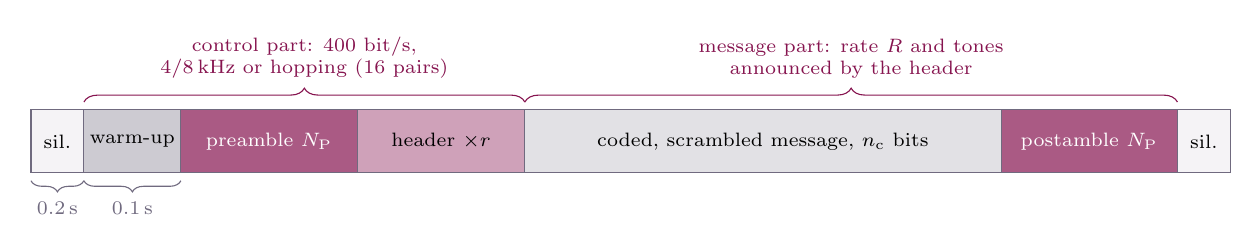
\begin{tikzpicture}[x=1.12cm,y=1cm, every node/.style={font=\scriptsize}]
\def\h{0.8}
\fill[iceground] (0,0) rectangle (0.6,\h); \node at (0.3,\h/2) {\scriptsize sil.};
\fill[icegrey!35] (0.6,0) rectangle (1.7,\h); \node at (1.15,\h/2) {warm-up};
\fill[icemagenta!70] (1.7,0) rectangle (3.7,\h); \node[white] at (2.7,\h/2) {preamble $\NP$};
\fill[icemagenta!40] (3.7,0) rectangle (5.6,\h); \node at (4.65,\h/2) {header $\times r$};
\fill[icegrey!20] (5.6,0) rectangle (11.0,\h); \node at (8.3,\h/2) {coded, scrambled message, $\nc$ bits};
\fill[icemagenta!70] (11.0,0) rectangle (13.0,\h); \node[white] at (12.0,\h/2) {postamble $\NP$};
\fill[iceground] (13.0,0) rectangle (13.6,\h); \node at (13.3,\h/2) {\scriptsize sil.};
\draw[icegrey] (0,0) rectangle (13.6,\h);
\foreach \x in {0.6,1.7,3.7,5.6,11.0,13.0} \draw[icegrey] (\x,0) -- (\x,\h);
\draw[decorate,decoration={brace,amplitude=5pt},icemagenta] (0.6,\h+0.1) -- (5.6,\h+0.1) node[midway,above=5pt,align=center] {control part: $400$ bit/s,\\$4/8\kHz$ or hopping (16 pairs)};
\draw[decorate,decoration={brace,amplitude=5pt},icemagenta] (5.6,\h+0.1) -- (13.0,\h+0.1) node[midway,above=5pt,align=center] {message part: rate $R$ and tones\\announced by the header};
\draw[decorate,decoration={brace,mirror,amplitude=4pt},icegrey] (0,-0.1) -- (0.6,-0.1) node[midway,below=4pt] {$0.2$\,s};
\draw[decorate,decoration={brace,mirror,amplitude=4pt},icegrey] (0.6,-0.1) -- (1.7,-0.1) node[midway,below=4pt] {$0.1$\,s};
\end{tikzpicture}
\caption{Frame layout (not to scale).}
\label{fig:frame}
\end{figure}

\paragraph{Warm-up.}
Forty alternating bits $1,0,1,0,\dots$ ($0.1$\,s at $400$ bit/s) precede the preamble.
They let the speaker's amplifier and the microphone's processing settle before the bits that matter.
With a hopping control part, the warm-up is numbered $k = -40, \dots, -1$, so that the preamble starts at symbol $k=0$ of the hopping pattern.

\paragraph{Duration.}
With $r$ copies of the 92-bit coded header,
\begin{equation}
D = \frac{40 + \NP + 92\,r}{\Rc} + \frac{\nc + \NP}{R} \quad (+\,0.4\text{ s of silence}).
\label{eq:duration}
\end{equation}
The control part lasts $0.65$, $1.20$ or $2.30$\,s for $\NP = 127$, $255$ or $511$.
\Cref{tab:durations} gives examples. With four tones, a frame lasts as long as with two at the same bit rate, up to a padding bit (\cref{sec:mfsk}).

\begin{table}[ht]
\centering
\caption{Frame duration $D$ in seconds from \cref{eq:duration} (preamble 127, without the silences). The 57-character text has $\nz = 456$ bits and the demo image ($74\times57$ pixels) $\nz = 4218$. $^{\ast}$Received only.}
\label{tab:durations}
\small
\begin{tabular}{llrrrrr}
\toprule
& & & \multicolumn{4}{c}{rate (bit/s)}\\
\cmidrule(lr){4-7}
Message & Code & $\nc$ & 200 & 400 & 800 & 1600\\
\midrule
text, 57 characters & none & 456 & 3.56 & 2.10 & 1.38 & 1.01\\
 & Hamming $(7,4)$ & 798 & 5.27 & 2.96 & 1.80 & 1.23\\
 & convolutional or turbo $1/2$ & 924 & 5.90 & 3.27 & 1.96 & 1.30\\
 & turbo $1/3$ & 1380 & 8.18 & 4.42 & 2.53 & 1.59\\
 & turbo $1/4$ & 1842 & 10.49 & 5.57 & 3.11 & 1.88\\
\midrule
demo image & none & 4218 & 22.37 & 11.51 & 6.08 & 3.36\\
 & Hamming $(7,4)$ & 7385 & 38.21 & 19.43 & 10.04 & 5.34\\
 & convolutional or turbo $1/2$ & 8448 & 43.52 & 22.09 & 11.37 & 6.01\\
 & turbo $1/3$ & 12666 & 64.61 & 32.63 & 16.64 & 8.64\\
 & turbo $1/4$ & 16890 & 85.73 & 43.19 & 21.92 & 11.28\\
 & Reed--Solomon$^{\ast}$ & 4992 & 26.24 & 13.45 & 7.05 & 3.85\\
\bottomrule
\end{tabular}
\end{table}

\subsection{Preambles: maximum-length sequences}
\label{sec:mls}
A maximum-length sequence (MLS, or m-sequence) of degree $m$ is the output of an $m$-stage linear feedback shift register whose feedback polynomial is primitive. It has period $N = 2^m - 1$ and contains $2^{m-1}$ ones~\cite{golomb}. Its antipodal version $a_j = 2b_j - 1$ has the two-valued periodic autocorrelation
\begin{equation}
\sum_{j=0}^{N-1} a_j\, a_{(j+\tau) \bmod N} = \begin{cases} N & \tau \equiv 0 \pmod N,\\ -1 & \text{otherwise,}\end{cases}
\label{eq:mlsacf}
\end{equation}
the closest a binary sequence can come to a single spike. This is why it is used as the preamble: its correlation peak locates the frame to within a fraction of a symbol, with low side lobes.
\begin{itemize}
\item $\NP = 127$: a fixed sequence inherited from version~0. It is the complement of the m-sequence that obeys $s_n = s_{n-6} \oplus s_{n-7}$ (characteristic polynomial $x^7 + x + 1$). Complementing changes the sign of $a_j$ only, so \cref{eq:mlsacf} still holds.
\item $\NP = 255$: Fibonacci LFSR with feedback polynomial $x^8 + x^6 + x^5 + x^4 + 1$, all-ones seed.
\item $\NP = 511$: polynomial $x^9 + x^5 + 1$, all-ones seed.
\end{itemize}
All three were checked to have the autocorrelation \cref{eq:mlsacf}. A longer preamble lets the frame be found farther away (\cref{sec:detect}), and the header is then repeated $r = 1, 2, 4$ times for $\NP = 127, 255, 511$, so that it can be read as far away as the frame is found.

\subsection{Header}
\label{sec:header}
The header carries 32 bits of information (\cref{tab:header}), most significant bit first, followed by an 8-bit cyclic redundancy check (CRC)~\cite{petersonbrown}.
\begin{table}[ht]
\centering
\caption{Header fields (32 bits, then CRC-8).}
\label{tab:header}
\begin{tabularx}{\linewidth}{lcX}
\toprule
Field & Bits & Meaning\\
\midrule
type & 2 & 0 text, 1 image, 2 room sounding\\
$a$ & 11 & text: number of characters; image: height $h$; sounding: MLS order\\
$b$ & 11 & text: 0; image: width $w$; sounding: number of periods\\
code & 2 & 0 none, 1 Hamming, 2 convolutional, 3 Reed--Solomon (turbo codes: see below)\\
rate & 2 & index into $\{200, 400, 800, 1600\}$ bit/s; with four tones, into $\{400, 800, 1600, 3200\}$; with tone set 3: 3 for 6400 bit/s, 0 and 1 for OFDM with the long and the short guard (version~3)\\
tones & 2 & 0 low ($4/8\kHz$), 1 high ($8/16\kHz$), 2 tone hopping, 3 four tones (version~2)\\
tone set & 2 & $0\,0$ (reserved before version~2); with four tones, 0 low, 1 high, 2 tone hopping, 3 the whole band (6400 bit/s, or OFDM)\\
CRC & 8 & generator $x^8 + x^2 + x + 1$, inverted for the turbo codes\\
\bottomrule
\end{tabularx}
\end{table}

\paragraph{CRC-8.}
With the 32 header bits as the coefficients of $m(x)$ (first bit = highest power), the check bits are the remainder
\begin{equation}
c(x) = x^8\, m(x) \bmod g(x), \qquad g(x) = x^8 + x^2 + x + 1,
\end{equation}
computed by a shift register with zero initial state and no final inversion. The same generator protects ATM cell headers~\cite{itui432}. The CRC rejects false detections and misread headers: a random 40-bit word passes the test (direct or inverted CRC, see below) with probability $2 \cdot 2^{-8} = 2^{-7}$, and the receiver additionally checks that the fields are valid (a text has at least one character and $b = 0$; an image has $1 \le h, w \le 256$ and $hw \le 20\,000$; a sounding has order 14, 15 or 16 and 1 to 8 periods).

\paragraph{Signalling the turbo codes by masking the CRC.}
The code field has only four values, all in use when the turbo code was added. The turbo codes of rate $1/2$, $1/3$ and $1/4$ (code numbers 4, 5 and 6) are therefore sent as codes 0, 1 and 2 with all eight CRC bits inverted. This is how 4G tells the number of transmit antennas, by masking the CRC of its broadcast channel~\cite{ts36212}. A receiver accepts a header if the CRC matches (codes 0--3) or matches after inversion (codes 4--7, of which 7 is unused). Receivers that predate the turbo code see a wrong CRC and ignore turbo frames instead of misdecoding them; receivers that predate rates $1/3$ and $1/4$ accept the inverted CRC but know no code 5 or 6, and ignore those frames too. Frames with the other codes are unchanged.

\paragraph{Signalling four tones (version~2).}
Four-tone frames set the tones field to 3, a value no earlier receiver accepts, and put their tone set in the two bits that were reserved; their rate field indexes $\{400, 800, 1600, 3200\}$ bit/s (\cref{sec:mfsk}). Versions~0 and~1 find no tone set~3 and ignore these frames. A version~2 receiver rejects a binary header whose last two bits are not $0\,0$, and a room sounding with tones field~3. Binary frames are unchanged. Tone set~3 with rate field~3 is 6400 bit/s (\cref{sec:wide}); receivers made before 6400 bit/s know no tone set~3 and ignore these frames.

\paragraph{Signalling OFDM (version~3).}
Tone set~3 with rate field~0 or~1 is OFDM with the long or the short guard (\cref{sec:ofdm}); rate field~2 is rejected. Receivers made before version~3 accept tone set~3 only with rate field~3 and ignore OFDM frames. The control part of an OFDM frame always hops.

\paragraph{Coding and repetition.}
The 40 bits go through the convolutional code of \cref{sec:conv}, with 6 tail bits: $2(40+6) = 92$ coded bits, sent $r$ times. The receiver adds the $r$ soft values of each coded bit before Viterbi decoding, which gains $10\log_{10} r$\,dB on the header (\cref{sec:hdrdec}).

\subsection{Message bits}
\begin{itemize}
\item \emph{Text}: each character is mapped to its Unicode code point if that is below 256 (Latin-1), else to \code{?}, and sent as 8 bits, most significant first. At most 1023 characters.
\item \emph{Image}: $h \times w$ black-and-white pixels (1 = white), column by column. The demo image is $74 \times 57$ pixels.
\item \emph{Room sounding}: no message bits; a waveform follows the control part (\cref{sec:sounding}).
\end{itemize}
The $\nz$ message bits are encoded by the code announced in the header (\cref{sec:codes}), giving $\nc$ coded bits, and then scrambled.

\subsection{Scrambler}
\label{sec:scrambler}
The coded bit $c_i$ is sent as $c_i \oplus k_i$, where $(k_i)$ is the output of the LFSR with polynomial $x^{15} + x^{14} + 1$ and all-ones seed: with state $s$ (15 bits), $k_i = s_{14} \oplus s_{13}$ and $s \leftarrow (2s + k_i) \bmod 2^{15}$. The sequence has period $2^{15} - 1 = 32\,767$. The same polynomial is used for energy dispersal in DVB~\cite{dvbs}.

The scrambler makes ones and zeros equally likely and breaks long runs of the same tone, whatever the message (an image is mostly white). This matters for the receiver: the calibration of \cref{sec:llr}, the levelling of \cref{sec:level} and the blind estimation of \cref{sec:em} all assume that both tones are used about equally often. The receiver undoes it on the soft values: $\lambda_i \leftarrow (-1)^{k_i} \lambda_i$.

%======================================================================
\section{Modulation: binary FSK on two fixed tones}
\label{sec:mod}
Symbol $k$ of a segment with rate $R$ is a burst of the tone $f_{b_k}$:
\begin{equation}
x[n] = 0.9\, \sin\!\left( 2\pi f_{b_k} \frac{n - kL}{\fsT} \right), \qquad kL \le n < (k+1)L, \quad L = \frac{\fsT}{R}.
\label{eq:fsk}
\end{equation}
The tone pairs are $(f_0, f_1) = (4, 8)\kHz$ (``low'', the default) or $(8, 16)\kHz$ (``high'', the tones of the original MATLAB demo). The amplitude $0.9$ leaves a small margin below digital full scale.

\paragraph{Orthogonality.}
Two tone bursts of duration $T$ are orthogonal for a non-coherent receiver, whatever their phases, when their frequencies differ by a multiple of $1/T$~\cite{proakis}. Here $(f_1 - f_0)T = 4000/R = 20, 10, 5$ at 200, 400, 800 bit/s for the low tones (and twice that for the high tones), so the detector at one tone sees nothing of the other. The exception is the low pair at 1600 bit/s, where $(f_1 - f_0)T = 2.5$: a burst at one tone then leaks into the other's detector with a relative amplitude $|\operatorname{sinc}(2.5)| = 1/(2.5\pi) \approx 0.13$, that is $-18\dB$.

\paragraph{No clicks.}
Every burst starts at phase 0 and $f_b T$ is a multiple of $\tfrac12$ for every tone and rate used, so every burst also ends at a zero crossing. The waveform is therefore continuous at the symbol boundaries (only its slope jumps), which limits the spectral splatter and the audible clicks.

%======================================================================
\section{Tone hopping}
\label{sec:hop}

\subsection{Why: the room's echo}
In a classroom, a tone keeps ringing after it stops: the reverberation time $T_{60}$ (the time for the sound energy to fall by $60\dB$) is typically $0.4$ to $1.2$\,s, hundreds of times the symbol duration. With two fixed tones, the echo of all the earlier bits sits on both tones. Beyond the \emph{critical distance}, where the direct sound is weaker than the reverberant field~\cite{kuttruff}, that echo is louder than the bit being read.

A simple model shows the effect. Let the reverberant energy decay as $e^{-t/\tau}$ with $\tau = T_{60}/(6\ln 10)$, and let each earlier symbol leave on its tone an echo proportional to that decay. With two fixed tones, each tone carried about half of the earlier symbols, so the echo energy on a tone during symbol $k$ is proportional to
\begin{equation}
\mathcal{E}_{\text{fixed}} \propto \frac12 \sum_{m\ge1} e^{-mT/\tau} = \frac{1}{2\,(e^{T/\tau} - 1)}.
\end{equation}
If instead each tone pair is used only once every $H$ symbols, the echo on the pair in use comes from symbols at least $HT$ in the past:
\begin{equation}
\mathcal{E}_{\text{hop}} \propto \frac12 \sum_{m\ge1} e^{-mHT/\tau} = \frac{1}{2\,(e^{HT/\tau} - 1)}, \qquad
\frac{\mathcal{E}_{\text{fixed}}}{\mathcal{E}_{\text{hop}}} = \frac{e^{HT/\tau} - 1}{e^{T/\tau} - 1} \ \ge\ H .
\label{eq:hopgain}
\end{equation}
The reduction is at least $H$ (the echo is spread over $2H$ tones instead of 2) and larger when $HT$ is comparable to $\tau$ (the echo has also decayed). \Cref{tab:hopgain} evaluates \cref{eq:hopgain}. The model ignores early reflections and the spectral leakage between tones, so it indicates a trend, not a measured gain. It also shows why, with hopping, slowing down helps again: a lower rate gives more pairs in the same band.

\begin{table}[ht]
\centering
\caption{Echo reduction on the tones in use, \cref{eq:hopgain}, in dB.}
\label{tab:hopgain}
\begin{tabular}{lcccc}
\toprule
Rate $R$ (bit/s) & 200 & 400 & 800 & 1600\\
Pairs $H$ & 32 & 16 & 8 & 4\\
\midrule
$10\log_{10} H$ & 15.1 & 12.0 & 9.0 & 6.0\\
$T_{60} = 0.6$\,s & 25.0 & 14.1 & 9.5 & 6.1\\
$T_{60} = 1.2$\,s & 19.5 & 13.0 & 9.3 & 6.1\\
\bottomrule
\end{tabular}
\end{table}

\subsection{Tone set and hopping pattern}
At $R$ bit/s the band $[3.2, 16)\kHz$ holds $H = 6400/R$ pairs of adjacent tones ($H = 32, 16, 8, 4$):
\begin{equation}
f_0^{(p)} = F_0 + 2pR, \qquad f_1^{(p)} = F_0 + (2p+1)R, \qquad p = 0, \dots, H-1, \qquad F_0 = 3200\Hz.
\label{eq:hoptones}
\end{equation}
Symbol $k$ of a segment uses the pair
\begin{equation}
p(k) = s\,k \bmod H, \qquad s = \frac{H}{2} - 1 .
\label{eq:hoppattern}
\end{equation}
Since $H$ is a power of two and $s$ is odd, $\gcd(s, H) = 1$ and each block of $H$ consecutive symbols visits every pair exactly once. Two consecutive symbols are $s$ pairs apart, $2sR = 6400 - 2R\Hz$ in frequency (6.0, 5.6, 4.8 and $3.2\kHz$ at 200 to 1600 bit/s), so the strongest early echo of a symbol, and any leakage due to a timing error, falls far from the next symbol's tones. \Cref{fig:hop} shows the pattern at 800 bit/s.

Counting of $k$: the control part counts from the first preamble bit (the warm-up has $k<0$); the message part counts from its first bit and continues through the postamble ($k = \nc, \dots, \nc + \NP - 1$); the postamble of a room sounding counts from its own first bit.

\begin{figure}[ht]
\centering
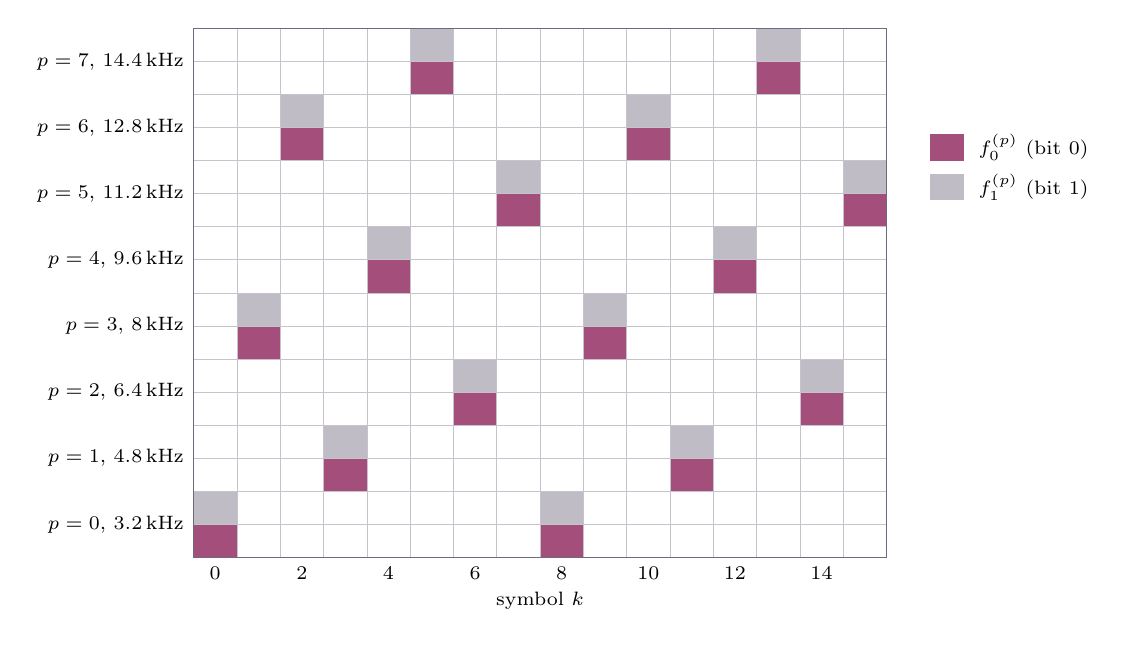
\begin{tikzpicture}[x=0.55cm,y=0.42cm, every node/.style={font=\scriptsize}]
\foreach \k in {0,...,15} {
  \pgfmathtruncatemacro{\p}{mod(3*\k,8)}
  \fill[icemagenta!75] (\k,2*\p) rectangle (\k+1,2*\p+1);
  \fill[icegrey!45] (\k,2*\p+1) rectangle (\k+1,2*\p+2);
}
\draw[step=1,icegrey!40,very thin] (0,0) grid (16,16);
\draw[icegrey] (0,0) rectangle (16,16);
\foreach \k in {0,2,...,14} \node[below] at (\k+0.5,0) {\k};
\node[below=9pt] at (8,0) {symbol $k$};
\foreach \p in {0,...,7} {
  \pgfmathsetmacro{\fa}{3.2+1.6*\p}
  \node[left] at (0,2*\p+1) {$p=\p$, \pgfmathprintnumber[fixed,precision=1]{\fa}\,kHz};
}
\fill[icemagenta!75] (17,12) rectangle (17.8,12.8); \node[right] at (17.9,12.4) {$f_0^{(p)}$ (bit 0)};
\fill[icegrey!45] (17,10.8) rectangle (17.8,11.6); \node[right] at (17.9,11.2) {$f_1^{(p)}$ (bit 1)};
\end{tikzpicture}
\caption{Tone hopping at 800 bit/s: $H = 8$ pairs between $3.2$ and $15.2\kHz$ ($f_1^{(p)} = f_0^{(p)} + 0.8\kHz$), pair $p(k) = 3k \bmod 8$. Each column shows the two tones available to symbol $k$; one of them is sent.}
\label{fig:hop}
\end{figure}

\paragraph{Orthogonality.}
All tones are multiples of $R$ ($F_0/R = 16, 8, 4, 2$), so each burst holds a whole number of cycles, and adjacent tones are $R = 1/T$ apart: the minimum spacing for orthogonal non-coherent FSK~\cite{proakis}. With correct timing, a burst produces no output at any other tone's detector.

\paragraph{Frame.}
A hopping message has a hopping control part (warm-up, preamble and header at 400 bit/s over 16 pairs, $3.2$ to $15.6\kHz$); otherwise far receivers, which tone hopping is meant for, would not even find the frame. The postamble hops at the message's rate. A room sounding requested with hopping uses the hopping control part and postamble. Version~0 receivers ignore hopping frames (tones field 2).

\paragraph{Why the band starts at 3.2\,kHz.}
The pairs first started at $1.6\kHz$. On a real 1600 bit/s recording, checked against the true bits, nearly all the channel errors came from the lowest pair: the $1.6\kHz$ tone was read wrong in 43\,\% of its symbols and its partner at $3.2\kHz$ in 8\,\%, against 0 to 0.2\,\% for every other pair. That tone arrived about $10\dB$ weaker than the tones from $4.8\kHz$ up (it is low in a small speaker's range), and the room's noise was concentrated below $2\kHz$, where the $1.6\kHz$-wide detector of a 1600 bit/s symbol collects it. Moving the band up by $1.6\kHz$ keeps its width, hence the number of pairs. In simulation (88 settings, 528 texts) 500 texts were read instead of 472. A side benefit: a harmonic of the bit-0 tone can land on its partner only if $f_0^{(p)} \le R$, which can no longer happen.

The idea of hopping FSK tones to escape reverberation is also used in underwater acoustic modems, where multipath is long compared with the symbols~\cite{kilfoyle,whoi}.

%======================================================================
\section{Four tones per symbol (version~2)}
\label{sec:mfsk}
Version~2 can send the message part with $M = 4$ tones per symbol (4-FSK) instead of two. Each symbol then carries $\log_2 M = 2$ bits. The control part is unchanged, binary at 400 bit/s, so every receiver still finds every frame and reads its header. On the page, the Transmit card's ``Modulation'' row chooses ``2 tones, 1 bit per symbol'' or ``4 tones, 2 bits per symbol''; in the script, \code{-{}-mod 4}.

\subsection{Why four tones}
At the same bit rate $R$, a four-tone symbol lasts $T_s = 2/R$, twice as long as a binary one, and its tones are spaced by the symbol rate $1/T_s = R/2$, the smallest orthogonal spacing (\cref{sec:mod}). Four tones therefore take the same band, $2R$, as a binary pair spaced by $R$. Three effects favour them.
\begin{itemize}
\item \emph{Energy per decision.} Each decision is made on twice the energy. For orthogonal signals detected non-coherently, the error probability per bit at a given energy per bit falls as $M$ grows, and the loss of non-coherent against coherent detection shrinks as the energy per decision grows~\cite{proakis}.
\item \emph{Echo.} With hopping, a group of tones is used again after $H$ symbols, that is after $2H/R$ seconds instead of $H/R$: its echo has decayed for twice as long (\cref{eq:hopgain} with $T$ doubled).
\item \emph{Timing.} A timing error of a given duration is a smaller fraction of a longer symbol. In the study that preceded version~2 (an ideal receiver, \code{mfsk\_study.md}), binary FSK at 3200 bit/s decoded only within $\pm 1/8$ of a binary symbol ($\pm 2$ samples at $48\kHz$) and had an error floor even close to the speaker, while four tones decoded within at least $\pm 1/2$.
\end{itemize}
The price is that each decision compares four energies: three tones that are not sent bring noise, instead of one. The same study found eight tones worth at most $1\dB$ more in noise, nothing in echo, and worse at 3200 bit/s, where their groups are too wide to hop well, so version~2 offers four.

\subsection{Mapping and tones}
The coded, scrambled bits are taken two at a time, and the pair $v = 2c_{2i} + c_{2i+1}$ selects the tone $m$ whose Gray code~\cite{gray} is $v$:
\begin{equation}
g(m) = m \oplus \lfloor m/2 \rfloor, \qquad m_i = g^{-1}(2c_{2i} + c_{2i+1}),
\label{eq:gray}
\end{equation}
so that tones $0, 1, 2, 3$ carry the pairs $00, 01, 11, 10$ (\cref{tab:gray}). Neighbouring tones, which leakage from a timing error mixes up most easily, differ in one bit only; in white noise, with orthogonal tones, all wrong tones are equally likely and the mapping does not matter. A message or postamble with an odd number of bits is padded with one 0. Each symbol is a burst of its tone as in \cref{eq:fsk}, with $L_s = 2\fsT/R$ samples (240, 120, 60, 30 at 400 to 3200 bit/s).

\begin{table}[ht]
\centering
\caption{Four-tone mapping and tones (version~2). With hopping, group $p = 0, \dots, H-1$, $H = 6400/R$, uses the pair $p$ of \cref{eq:hoptones} and the two tones halfway above each of its tones.}
\label{tab:gray}
\small
\begin{tabular}{ccccc}
\toprule
Tone $m$ & bits $c_{2i}\,c_{2i+1}$ & low & high & hopping, group $p$\\
\midrule
0 & 0\,0 & $4.0\kHz$ & $8.0\kHz$ & $F_0 + 2pR$\\
1 & 0\,1 & $5.6\kHz$ & $9.6\kHz$ & $F_0 + 2pR + R/2$\\
2 & 1\,1 & $7.2\kHz$ & $11.2\kHz$ & $F_0 + (2p+1)R$\\
3 & 1\,0 & $8.8\kHz$ & $12.8\kHz$ & $F_0 + (2p+1)R + R/2$\\
\bottomrule
\end{tabular}
\end{table}

\paragraph{Fixed tones.}
The fixed sets start at the lower tone of the binary pairs, 4 or $8\kHz$, with a spacing of $1.6\kHz$, the symbol rate at 3200 bit/s: $\Delta f\,T_s = 3200/R = 8, 4, 2, 1$ at 400 to 3200 bit/s, so the four tones are orthogonal at every rate (unlike the binary $4/8\kHz$ pair at 1600 bit/s, \cref{sec:mod}). At 6400 bit/s they would not be ($\Delta f\,T_s = 1/2$), so that rate has tones of its own (\cref{sec:wide}). The low set, 4 to $8.8\kHz$, stays where small speakers and phone microphones are good.

\paragraph{Hopping.}
The $H = 6400/R$ pairs of \cref{eq:hoptones} become $H$ groups of four tones, $f_m^{(p)} = F_0 + 2pR + mR/2$, in the same band and with the same pattern \cref{eq:hoppattern}, symbols counted as in \cref{sec:hop}. The top tone is at 15.8, 15.6, 15.2 and $14.4\kHz$ at 400 to 3200 bit/s. At 3200 bit/s there are only $H = 2$ groups, used in turn, and at 6400 bit/s a single one (\cref{sec:wide}). Every tone is a multiple of $R/2$, so each burst holds a whole number of cycles; with fixed tones, $f T_s$ is a multiple of $\tfrac12$. As in version~1, every burst therefore starts and ends at a zero crossing.

\paragraph{Frame.}
The $\nc$ coded bits become $n_s = \lceil \nc/2 \rceil$ symbols and the postamble $\lceil \NP/2 \rceil$ symbols (64, 128 or 256), whose known tones are given by the preamble's bits taken in pairs with a 0 appended. The duration \cref{eq:duration} becomes
\begin{equation}
D = \frac{40 + \NP + 92\,r}{\Rc} + \frac{2\,\bigl(\lceil \nc/2 \rceil + \lceil \NP/2 \rceil\bigr)}{R} \quad (+\,0.4\text{ s of silence}),
\end{equation}
nearly the same as with two tones at the same bit rate. At 3200 bit/s with the 127-bit preamble, the 57-character text with the convolutional code lasts $0.98$\,s and the demo image $3.33$\,s.

\subsection{Receiver}
\label{sec:mfskrx}
The receiver is that of \cref{sec:rx}, with symbols in place of bits in the message part: windows of $W = \round{2\fs/R}$ samples, instants $t_j$ (\cref{sec:clock}) one symbol, $2\fs/R$ samples, apart, and four energies $E_{m,j}$ per symbol. The steps that compare tones are generalised so that with $M = 2$ each one reduces to its version-1 formula: the version-2 page and script decode binary frames to the same bits as version~1, apart from the narrower postamble search.

\paragraph{Soft output.}
Calibration (\cref{eq:cal}) is done per tone: $P_{\text{on},m}$ is the mean of $E_m^2$ over the postamble symbols that send tone $m$, about a quarter of them, and $P_{\text{off},m}$ over the others. With the tones independent given the symbol,
\begin{equation}
\ln p(\bm E \mid m) = \lambda_m + \sum_{m'=0}^{M-1} \ln p_{\text{off},m'}(E_{m'}), \qquad
\lambda_m = \ln \frac{p_{\text{on},m}(E_m)}{p_{\text{off},m}(E_m)} = \ln I_0\!\Bigl(\frac{A_m E_m}{\sigma_m^2}\Bigr) - \frac{A_m^2}{2\sigma_m^2},
\end{equation}
where the sum is the same for every $m$. With equally likely symbols (the scrambler), the LLR of bit $i$ of the symbol is
\begin{equation}
\lambda^{(i)} = \ln \sum_{m:\, g_i(m) = 1} e^{\lambda_m} \;-\; \ln \sum_{m:\, g_i(m) = 0} e^{\lambda_m},
\label{eq:bicm}
\end{equation}
with $g_i(m)$ bit $i$ of the Gray code of $m$: the bit metric of bit-interleaved coded modulation~\cite{bicm}. For $M = 2$ it is $\lambda_1 - \lambda_0$, \cref{eq:llr}. The decoders treat the two LLRs of a symbol as independent, the usual approximation of bit-interleaved coded modulation; the interleaver of \cref{sec:ilv} places them far apart in the codeword. The plain ratio becomes $\ln\bigl((\max_{g_i(m)=1} E_m + \epsilon)/(\max_{g_i(m)=0} E_m + \epsilon)\bigr)$, the strongest tone whose bit is 1 against the strongest whose bit is 0. The scale $\alpha$ (\cref{eq:alpha}) is fitted on the $2\lceil \NP/2 \rceil$ bit LLRs of the postamble. In the blind estimation (\cref{sec:em}) the weights become the probabilities of the four tones, $w_{m,j} = e^{\lambda_{m,j}} / \sum_{m'} e^{\lambda_{m',j}}$, starting from the strongest tone, and each tone's energies count as on with weight $w_{m,j}$ and as off with $1 - w_{m,j}$. The level tracking uses $q_i = \max_m E_{m,i}^2/\hat A_m^2$, and the errors on the postamble are counted in bits, from the strongest tone of each symbol.

\paragraph{Tone levelling (hopping).}
With two tones, \cref{sec:level} divides each tone's energies by their rms over the symbols of its pair, in about half of which the tone is sent. With four tones a tone is sent in only a quarter of its group's symbols. In a 57-character text at 400 bit/s, each tone of a group is sent about 8 times, a number that varies by about 30\,\% from tone to tone: too few symbols for the rms to measure the same mixture of signal and noise for every tone (a tone never sent in a group would have its noise raised to the level of the others). In simulation this caused errors at 400 bit/s even without noise. The level of tone $m$ in group $p$ is therefore measured where that tone was most probably sent,
\begin{equation}
g_{m,p} = \sqrt{\frac{1}{|\mathcal K_{m,p}|} \sum_{k \in \mathcal K_{m,p}} E_{m,k}^2}, \qquad \mathcal K_{m,p} = \bigl\{k : p(k) = p,\ \arg\max_{m'} E_{m',k} = m\bigr\},
\end{equation}
over the message and the postamble, or, if $\mathcal K_{m,p}$ is empty, as the rms of the strongest energy over all the group's symbols.

\paragraph{Contrast.}
The early--late gate, the fine timing and its $t$-test (\cref{sec:track,sec:finetiming}) use the contrast of a symbol, $d = (E_{(1)} - E_{(2)})/\sum_m E_m$ with $E_{(1)} \ge E_{(2)}$ its two largest energies, which is $|E_1 - E_0|/(E_1 + E_0)$ for two tones. The postamble correlator uses how much the known tone $s$ stands out,
\begin{equation}
\kappa_s(\bm E) = \frac{M E_s - \sum_m E_m}{(M - 1) \sum_m E_m}, \qquad c(m) = \frac{1}{n_{\mathrm P}} \sum_{j=0}^{n_{\mathrm P} - 1} \kappa_{s_j}\bigl(\bm E(m + o_j)\bigr),
\end{equation}
which is 1 when only tone $s$ is heard, $-1/(M-1)$ when only it is silent and about 0 in noise; for two tones $\kappa_{s_j} = a_j d$, the correlator of \cref{sec:detect}. Here $n_{\mathrm P}$ is the number of postamble symbols and $o_j$ the offset of symbol $j$. The fine timing works on blocks of symbols, with $\epsilon_{\max} = \min\bigl(\lfloor \fs/R \rfloor, \round{0.5\ms \cdot \fs}\bigr)$, half a symbol at most.

\paragraph{Results.}
In simulation (\cref{tab:mfsk}), at the same bit rate, four tones tolerated about $2\dB$ more noise and, for 9 texts in 10, 2 to $3\dB$ more echo than two. Four tones at $2R$, twice the throughput of two tones at $R$, needed only $0.6$ to $0.9\dB$ more SNR but about $2\dB$ more DRR.

\subsection{6400 bit/s: one group over the whole band}
\label{sec:wide}
At $R = 6400$ bit/s the hopping rule gives $H = 6400/R = 1$: a single group of four tones $f_m = F_0 + mR/2 = 3.2, 6.4, 9.6, 12.8\kHz$, spaced by the symbol rate of 3200 symbols/s, with symbols of $T_s = 0.31\ms$ ($L_s = 15$ samples at $48\kHz$). The group fills the band, so there is nothing left to hop over. This is as fast as orthogonal FSK goes in a band $B$: $M$ tones spaced by the symbol rate $R_s$ take $B = M R_s$ and carry $R = R_s \log_2 M$, so
\begin{equation}
\frac{R}{B} = \frac{\log_2 M}{M} \le \frac12 \ \text{bit/s per Hz},
\end{equation}
with equality for $M = 2$ and $M = 4$: 6400 bit/s in the $12.8\kHz$ from 3.2 to $16\kHz$. Going further takes many tones at once, each with its own phase, as in OFDM.

\paragraph{Frame.}
The header sends tone set~3 with rate field~3 (\cref{sec:header}). The page offers 6400 bit/s only with four tones and selects hopping with it; the script requires \code{-{}-tones hop}. The control part still runs at 400 bit/s and becomes a large share of a fast frame: with the 127-bit preamble, the 57-character text with the convolutional code lasts $0.81$\,s and the demo image $1.99$\,s, of which $0.65$\,s are preamble and header.

\paragraph{Receiver.}
It is the hopping receiver with one group, except for the postamble's threshold. Since every symbol uses the same four tones, the early reflections, a few milliseconds or tens of symbols long, fall on the tones of the following symbols, and the postamble correlation $c(p_2)$ stays near $0.39$ in the model room even with little reverberation ($0.69$ at 3200 bit/s), below half of the preamble's (about $0.8$ to $0.94$). The postamble is therefore declared found from a fifth of $c(p_1)$; its side lobes, a symbol or more from the peak, stay near $0.02$. With half, it was never found at 6400 bit/s; with a fifth, it was found in 14 to 16 of 16 frames from DRR $-3\dB$ up, and the texts were read about as often as with the blind calibration (within 2 in 16).

\begin{table}[ht]
\centering
\caption{3200 against 6400 bit/s with four tones (tone hopping, a single group at 6400 bit/s; otherwise as in \cref{tab:mfsk}): the SNR (noise, DRR $+6\dB$) and the DRR (echo, SNR $40\dB$) at which half, and 9 in 10, of the texts are read, and the cost of 6400 bit/s in dB.}
\label{tab:wide}
\small
\begin{tabular}{rcc}
\toprule
bit/s & noise: SNR (dB) & echo: DRR (dB)\\
\midrule
3200 & $-1.7$ / $-0.7$ & $-5.2$ / $-3.5$\\
6400 & $+3.0$ / $+3.8$ & $-1.6$ / $-0.5$\\
cost & 4.7 / 4.5 & 3.6 / 3.0\\
\bottomrule
\end{tabular}
\end{table}

\paragraph{Results.}
6400 bit/s needed $4.5$ to $4.7\dB$ more SNR and 3 to $3.6\dB$ more DRR than 3200 bit/s (\cref{tab:wide}). Each earlier doubling of the four-tone bit rate cost about $3\dB$; in noise this one costs more, because the echo of the earlier symbols, always on the same four tones, adds to the noise. By the rule of $6\dB$ per doubling of the distance, 6400 bit/s reaches roughly 60 to 70\,\% of the distance of 3200 bit/s. A clock offset of $\pm 50$\,ppm and a $44.1\kHz$ microphone changed the counts by at most 2 texts in 16.

\paragraph{Beyond 6400 bit/s.}
A wider band, up to $20\kHz$ if the phones and the laptop reproduce it, would add about 30\,\%. Beyond that comes OFDM, many tones at once with a phase on each. A simulation study in the same room model (\code{ofdm\_study.md}: DQPSK on 546 subcarriers from 3.2 to $16\kHz$, symbols of 64\,ms with a 21\,ms cyclic prefix, peaks clipped $6\dB$ above the rms) found that in echo it carries about 2.7 times the information rate of FSK for $1\dB$ less range: 4.3\,kbit/s with the rate-$1/4$ turbo code down to DRR $-4.3\dB$, against $-5.2\dB$ for FSK at 3200 bit/s (1.6\,kbit/s). In noise it is worse: 4.3\,kbit/s needed an SNR of $+6.0\dB$, $3\dB$ more than FSK at 6400 bit/s (3.2\,kbit/s), because it plays $3.4\dB$ quieter for the same peaks and differential detection costs about $3\dB$. A phone moving at 0.1\,m/s scales time by 300\,ppm, which breaks OFDM unless the receiver estimates the scale and resamples the recording. Where 3200 bit/s just stops working (DRR about $-5\dB$), Shannon's capacity $B \log_2(1 + \mathrm{SINR})$, with the late echo counted as noise, is about 5\,kbit/s of information (an estimate). Version~3 builds this OFDM mode (\cref{sec:ofdm}). With the real receiver the study's thresholds held within $0.5\dB$ in the same room model, but in a room whose echo is diffuse from the start the gain in echo is smaller (\cref{sec:ofdmres}).

%======================================================================
\section{OFDM (version~3)}
\label{sec:ofdm}
Version~3 adds a third modulation for the message part: orthogonal frequency-division multiplexing (OFDM)~\cite{weinstein}, many subcarriers at once, each with its own phase, as in Wi-Fi~\cite{ieee80211} and digital radio~\cite{dab}. The control part is the hopping one (400 bit/s, \cref{sec:hop}), so every receiver finds the frame and reads its header; receivers older than version~3 then ignore the frame (\cref{sec:header}). On the page, the Modulation row has a third button, ``OFDM'', which replaces the Tones and Rate rows by a ``Guard interval'' row; in the script, \code{-{}-mod ofdm -{}-guard long} or \code{short}.

\subsection{Why OFDM}
FSK sends one tone at a time and carries at most half a bit per second per hertz (\cref{sec:wide}). At high rates its symbols are a fraction of a millisecond long, and the room's echo of earlier symbols is what limits it. OFDM instead puts one complex number on each of $K$ subcarriers of a long symbol and repeats the end of the symbol before it, as a cyclic prefix or \emph{guard interval}. An echo that arrives within the guard then turns into a single complex gain per subcarrier, the room's frequency response at that frequency, and the symbols no longer overlap. With two bits per subcarrier, OFDM approaches 2 bit/s per hertz, less the share of time spent on the guard.

\subsection{Subcarriers and symbols}
With an FFT of $N$ points at $\fsT$, subcarrier $k$ is at $k\,\fsT/N$, and the subcarriers used are those from 3.2 to $16\kHz$,
\begin{equation}
\mathcal K = \{k_0 < k_1 < \dots < k_{K-1}\} = \bigl\{k : 3200\,N \le k\,\fsT < 16\,000\,N\bigr\}.
\end{equation}
Symbol $i$ is, for $n = -C, \dots, N - 1$ (the first $C$ samples are the guard, a copy of the last $C$),
\begin{equation}
x_i[n] = a \sum_{j=0}^{K-1} \cos\!\Bigl(\frac{2\pi k_j n}{N} + \varphi_{i,j}\Bigr), \qquad a = 0.45\sqrt{2/K},
\label{eq:ofdmsym}
\end{equation}
computed as an inverse real FFT. Its rms is $a\sqrt{K/2} = 0.45$, half the $0.9$ peak of FSK, and samples beyond $\pm 0.9$ are clipped. Two choices of $N$ and $C$ are offered (\cref{tab:ofdm}); the header says which.

\begin{table}[ht]
\centering
\caption{The two OFDM modes (version~3). Bit rates before the code are $2K\fsT/(N+C)$.}
\label{tab:ofdm}
\small
\setlength{\tabcolsep}{4.5pt}
\begin{tabular}{lcccccccc}
\toprule
Guard & $N$ & $C$ & guard & symbol + guard & $K$ & spacing & before the code & turbo $1/2$ / $1/4$\\
\midrule
long & 2048 & 1024 & $21.3\ms$ & $64.0\ms$ & 546 & $23.4\Hz$ & 17.1\,kbit/s & 8.5 / 4.3\,kbit/s\\
short & 1024 & 256 & $5.3\ms$ & $26.7\ms$ & 273 & $46.9\Hz$ & 20.5\,kbit/s & 10.2 / 5.1\,kbit/s\\
\bottomrule
\end{tabular}
\end{table}

\paragraph{Why the guard works.}
Let the room's response $h$ have its paths at delays $d \in [\tau, \tau + C]$ samples, and let the receiver take the FFT of the $N$ samples that start $C + \tau$ samples after symbol $i$ begins. Every path then contributes a whole period of the same symbol, cyclically shifted, so the window holds the circular convolution of $x_i$ with $h$. Its DFT at subcarrier $k_j$ is
\begin{equation}
Y_{i,j} = \frac{N a}{2}\, H_j\, e^{j\varphi_{i,j}} + w_{i,j},
\label{eq:ofdmrx}
\end{equation}
with $H_j$ the room's response at subcarrier $j$ (including the phase of the window's position) and $w_{i,j}$ the noise. Paths outside $[\tau, \tau + C]$ leak the previous or the next symbol into the window and act as noise; that is why the guard must outlast most of the room's echo, and why the short guard, $5.3\ms$, loses more in reverberant rooms.

\subsection{Differential QPSK}
\label{sec:dqpsk}
The receiver does not estimate $H_j$: each subcarrier carries two bits as the phase step from one symbol to the next (DQPSK), as in DAB~\cite{dab}. The coded, scrambled bits of data symbol $i = 1, \dots, n_s$ on subcarrier $j$ are $b_0 = c_{2((i-1)K + j)}$ and $b_1 = c_{2((i-1)K + j) + 1}$, the last symbol padded with zeros, and
\begin{equation}
\varphi_{i,j} = \theta_j + \frac{\pi}{4} P_{i,j}, \qquad P_{i,j} = \bigl(P_{i-1,j} + 1 + 2\,[(b_0 \oplus b_1) + 2 b_1]\bigr) \bmod 8, \qquad P_{0,j} = 0.
\label{eq:dqpsk}
\end{equation}
The steps $\pi/4$, $3\pi/4$, $5\pi/4$, $7\pi/4$ carry $00$, $10$, $11$, $01$: a Gray mapping in which the sign of the real part of the step gives $b_0$ and that of its imaginary part $b_1$. Symbol $0$ and symbol $n_s + 1$ are the reference symbol, $P = 0$ on every subcarrier, with the phases
\begin{equation}
\theta_j = \frac{\pi\,(j^2 \bmod 2K)}{K},
\end{equation}
Newman's phases for a multitone with a low crest factor~\cite{boyd}: its peaks are $5.4\dB$ above its rms (0.84), so it is never clipped. The data symbols have nearly Gaussian samples: $4.5\,\%$ of them exceed $0.9$ and are clipped, which leaves the clipping noise $19\dB$ below the signal. With the same peaks, OFDM plays $3\dB$ quieter than FSK, whose rms is $0.9/\sqrt2$.

\subsection{Frame}
The frame is the hopping control part (warm-up, preamble, header) followed by the reference symbol, the
\begin{equation}
n_s = \Bigl\lceil \frac{\nc}{2K} \Bigr\rceil
\end{equation}
data symbols and the reference symbol again, each with its guard; there is no postamble. The header has tone set~3 and the rate field 0 for the long guard, 1 for the short one (\cref{sec:header}). The duration \cref{eq:duration} becomes
\begin{equation}
D = \frac{40 + \NP + 92\,r}{\Rc} + \frac{(n_s + 2)(N + C)}{\fsT} \quad (+\,0.4\text{ s of silence}).
\end{equation}
With the 127-bit preamble, the 57-character text with the convolutional code ($n_s = 1$) lasts $0.84$\,s, of which $0.65$\,s is the control part; the demo image lasts $1.29$\,s with turbo $1/2$ ($n_s = 8$), $1.80$\,s with turbo $1/4$ and $1.13$\,s with the short guard and turbo $1/2$, against $1.99$\,s with FSK at 6400 bit/s.

\subsection{Receiver}
\label{sec:ofdmrx}
Once the header is read, the receiver waits until the whole OFDM part should be in, with $0.1\,\%$ to spare, and processes it in one go (\code{ofdmReceive} in the page, \code{ofdm\_receive} in the script, which give the same results). The preamble's position $p_1$ predicts the start of the first guard, $t_0 = p_1 + (\NP + 92\,r)\,\fs/\Rc$ in the recording's samples.

\paragraph{1. Reading on the transmitter's grid.}
Whatever the microphone's rate, the OFDM part is read at the instants $t_0 + m\,(\fs/\fsT)(1 + \varepsilon)$, $m = -N/2, \dots, (n_s + 2)(N + C) + N/2$, by windowed-sinc interpolation,
\begin{equation}
r[m] = \sum_{|u| < A} y[q]\,\operatorname{sinc}(u)\,\tfrac12\bigl(1 + \cos(\pi u/A)\bigr), \qquad u = t_m - q,\ A = 16,
\end{equation}
first with $\varepsilon = 0$. This turns the recording into samples at $48\kHz$, the transmitter's rate, on which the FFTs of $N$ points line up with the subcarriers.

\paragraph{2. Timing from the reference symbol.}
The receiver takes the FFT of the reference symbol's window starting in the middle of its guard, removes the known phases and tapers the band with a Hann window $w_j$ (lower side lobes in time):
\begin{equation}
g[n] = \Bigl|\sum_{j} Y_{0,j}\, e^{-j\theta_j}\, w_j\, e^{j 2\pi k_j n/N}\Bigr|^2, \qquad n = 0, \dots, N - 1.
\end{equation}
This is the room's impulse response as seen in the band, a path of delay $d$ (from $t_0$) at index $C/2 + d$, modulo $N$. The receiver looks for the stretch of $C + 1$ indices, starting at $s$ within $C/2 \pm N/4$, that holds the most energy, $E(s) = \sum_{n=s}^{s+C} g[n \bmod N]$, and takes the latest $s$ with $E(s) \ge 0.99 \max E$: the direct sound then sits at the start of the stretch and the guard covers as much of the later echo as possible. The timing correction is $\tau = s - C/2$.

\paragraph{3. Time scale.}
A clock offset between the two devices, or a phone moving at $v$ (a scale of $v/c$: $290$\,ppm at $0.1$\,m/s), stretches the recording by a factor $1 + \varepsilon$. Symbol $i$ then arrives $i(N + C)\varepsilon$ samples late, which turns subcarrier $f$ by $2\pi f\, i(N + C)\varepsilon/\fsT$. Between two consecutive long-guard symbols this is $18^\circ$ at $16\kHz$ for $50$\,ppm and $111^\circ$ for 300\,ppm, against the $45^\circ$ margin of DQPSK: without a correction, a moving phone could not read OFDM. The two reference symbols, $(n_s + 1)(N + C)$ samples apart, give the receiver
\begin{equation}
z_j = Y_{n_s+1,j}\, Y_{0,j}^{*}, \qquad \hat\varepsilon = \arg\max_{|\varepsilon| \le 500\,\mathrm{ppm}} \Bigl|\sum_j z_j\, e^{\,j 2\pi f_j (n_s + 1)(N + C)\varepsilon/\fsT}\Bigr|,
\label{eq:ofdmeps}
\end{equation}
searched in steps of 1\,ppm and refined by a parabola through the peak and its neighbours. Both windows start in the middle of their guards, $C/2 + \tau$, so that a drift of up to $C/2$ samples between the references keeps both inside their guards (at 500\,ppm, up to $n_s = 332$ with the long guard and 199 with the short one, more than the largest image needs). If $|\hat\varepsilon| > 0.05$\,ppm, the part is read again with $\varepsilon = \hat\varepsilon$, and the timing of step~2 is found again on both reference symbols, now aligned.

\paragraph{4. Windows.}
The data windows start $C + \tau - 8$ samples after each symbol's start: the 8 samples of margin keep the direct sound inside the guard if the timing is slightly late, at the cost of 8 samples of late echo. The receiver also computes $g$ for these windows on both references: the share of its energy in indices $0$ to $C$ is the energy that arrives within the guard, and the page plots it (\cref{sec:ofdmshow}).

\paragraph{5. Differential detection and LLRs.}
On each subcarrier, $z_{i,j} = Y_{i,j} Y_{i-1,j}^{*}$ for $i = 1, \dots, n_s$. With \cref{eq:ofdmrx}, $z_{i,j} \approx |N a H_j/2|^2\, e^{j(\varphi_{i,j} - \varphi_{i-1,j})}$ plus noise: the room's response cancels. Writing $A_j = |N a H_j/2|$ and $\sigma_j^2$ for the variance of $w_{i,j}$, each component of the noise on $z$ has a variance of about $A_j^2 \sigma_j^2$ (neglecting $w_i w_{i-1}^*$), and the QPSK points are at $A_j^2(\pm 1 \pm j)/\sqrt2$, so that
\begin{equation}
\lambda(b_0) = -\frac{\sqrt2\, \operatorname{Re} z_{i,j}}{N_{0,j}}, \qquad \lambda(b_1) = -\frac{\sqrt2\, \operatorname{Im} z_{i,j}}{N_{0,j}}, \qquad N_{0,j} = \sigma_j^2,
\end{equation}
positive for a 1, as in \cref{sec:llr}. The noise is estimated per group $G$ of 32 subcarriers, across the decisions $\hat d = (\operatorname{sign}\operatorname{Re} z + j \operatorname{sign}\operatorname{Im} z)/\sqrt2$:
\begin{equation}
N_{0,G} = \frac{\operatorname{mean}_{i,\, j \in G} \bigl(\operatorname{Im}(z_{i,j}\, \hat d_{i,j}^{*})\bigr)^2}{\operatorname{mean}_{i,\, j \in G}\, \tfrac12\bigl(|Y_{i,j}|^2 + |Y_{i-1,j}|^2\bigr)},
\qquad \mathrm{SNR}_G = \frac{\operatorname{mean} \tfrac12\bigl(|Y_{i,j}|^2 + |Y_{i-1,j}|^2\bigr)}{N_{0,G}} - 1.
\end{equation}
It includes the echo that arrives outside the guard, the clipping noise and whatever the time-scale estimate left. These LLRs go to the decoder (\cref{sec:decode}), whichever soft output is chosen on the page; the scrambler is undone on them as for FSK.

\paragraph{What the page shows.}
\label{sec:ofdmshow}
The impulse response of step~4 in dB, with the guard shaded (echo inside it is harmless, echo after it is noise), the share of the energy after the guard, the SNR per subcarrier (lowest, highest, median over the groups), the clock offset $\hat\varepsilon$, and $\tau$.

\subsection{Results}
\label{sec:ofdmres}
\Cref{tab:ofdmres} compares OFDM and FSK in simulation (57-character text, preamble 511, $T_{60} = 0.6$\,s, the script's receiver) in two model rooms. Room~A is the model with early reflections used for the other tables: direct sound, four reflections between 3 and $14\ms$, a diffuse tail and a speaker filter; its DRR counts the reflections as echo. Room~B is the script's simulator (\cref{sec:roomsim}): a direct sound followed by a diffuse tail from $1\ms$ on.

\begin{table}[ht]
\centering
\caption{OFDM against four-tone FSK (hopping): the DRR at SNR $40\dB$ (echo) and the SNR at DRR $+6\dB$ in room~A (noise, set relative to a 3200 bit/s FSK frame, so the same for every frame) at which half of the texts are read. Room~A: 16 trials per point, $1\dB$ grid; room~B: 8 trials, $2\dB$ grid, interpolated.}
\label{tab:ofdmres}
\small
\begin{tabular}{lcccc}
\toprule
& message & echo, room A & echo, room B & noise, room A\\
& bit/s & DRR (dB) & DRR (dB) & SNR (dB)\\
\midrule
FSK 3200 bit/s, turbo $1/2$ & 1.6\,k & $-5.2$ & $-5.0$ & $-1.7$\\
FSK 6400 bit/s, turbo $1/2$ & 3.2\,k & $-1.6$ & $-1.6$ & $+3.0$\\
OFDM long guard, turbo $1/4$ & 4.3\,k & $-4.4$ & $-1.3$ & $+5.5$\\
OFDM long guard, turbo $1/2$ & 8.5\,k & $-0.5$ & $+3.1$ & $+9.4$\\
OFDM short guard, turbo $1/2$ & 10.2\,k & $+1.3$ & $+5.3$ & $+10.7$\\
\bottomrule
\end{tabular}
\end{table}

\begin{itemize}
\item \emph{Echo.} FSK does not care how the echo is spread in time, and the two rooms give it the same thresholds. OFDM does: in room~A part of the echo is the early reflections, which fall inside the guard and do no harm, so OFDM gains 3 to $4\dB$ over room~B. With turbo $1/4$ it carries 4.3\,kbit/s, $1.3$ times FSK at 6400 bit/s, as far as FSK at 6400 bit/s (room~B) or nearly as far as FSK at 3200 bit/s (room~A). The short guard needs about $2\dB$ more than the long one in both rooms for $20\,\%$ more bit rate.
\item \emph{Noise.} With turbo $1/4$, OFDM needs $2.5\dB$ more than FSK at 6400 bit/s: it plays $3\dB$ quieter, and differential detection costs about $3\dB$ against coherent detection, while FSK's four tones gain from their long decisions (\cref{sec:mfsk}).
\item \emph{Time scale.} With $\pm 300$\,ppm, or a $44.1\kHz$ microphone with $\pm 50$\,ppm, the counts were the same as with none (long guard, turbo $1/4$, DRR $-4$ and $-3\dB$ in room~A: 13 and 16 of 16; turbo $1/2$ and the short guard at $+1\dB$: 16 and 4 of 16).
\item The study that preceded version~3 (\code{ofdm\_study.md}: room~A, perfect timing and time scale) found the same thresholds within $0.5\dB$, so steps 2 and~3 cost little.
\end{itemize}

\paragraph{The real recording.}
From the decoded image of the 1600 bit/s recording (\cref{sec:results}), the frame that was sent can be rebuilt and compared with what the phone heard, by least squares over the frame. In 1.6 to $14\kHz$, $81\,\%$ of the received energy arrived within $1\ms$ of the direct sound, $16\,\%$ between 1 and $5.3\ms$, $1\,\%$ between 5.3 and $21.3\ms$ and about $1\,\%$ later: at that spot, even the short guard would have held nearly all the echo. The background noise was $36\dB$ below the signal in 3.2 to $16\kHz$, and the delay changed by less than $0.1$ sample per $64\ms$ (20\,ppm) most of the time, and by up to $0.6$ sample (about 200\,ppm, a few centimetres per second) for about a second. Yet only 55 to $80\,\%$ of the received energy in 3.2 to $16\kHz$ was a linear echo of what was sent; the rest, 1 to $6\dB$ below the signal, was neither echo nor background noise. Distortion in the speaker or the microphone is the likely cause (an inference, not a measurement): all the tones of that frame were multiples of $1.6\kHz$, so their harmonics fall on other tones, and the second harmonic of $1.6\kHz$ is $3.2\kHz$, the other tone of its pair, which fits the $43\,\%$ of 0s read as 1s on that pair. For OFDM such distortion acts as noise, where it needs more signal than FSK; at that spot, FSK at 3200 bit/s should reach farther than OFDM. With $36\dB$ of margin above the background noise, a lower volume may lower the distortion more than the signal.

%======================================================================
\section{Channel codes}
\label{sec:codes}
The code is chosen on the transmitter and announced in the header. \Cref{tab:codes} summarises the codes; their lengths are such that a frame lasts exactly as long with the convolutional code and the rate-$1/2$ turbo code.

\begin{table}[ht]
\centering
\caption{Codes, for $\nz$ message bits. Hamming, convolutional and turbo codewords then go through the interleaver of \cref{sec:ilv}.}
\label{tab:codes}
\begin{tabularx}{\linewidth}{lllX}
\toprule
Code & Rate & Coded length $\nc$ & Decoder\\
\midrule
none & 1 & $\nz$ & sign of the LLR\\
Hamming $(7,4)$ & $4/7$ & $7\lceil \nz/4 \rceil$ & syndrome, hard decisions\\
convolutional $(171,133)_8$, $K=7$ & $\approx 1/2$ & $2(\nz + 6)$ & soft-decision Viterbi\\
turbo, $(1, 15/13)_8$ RSC $\times 2$ & $\approx 1/2$ & $2\nz + 12$ & iterative log-MAP, $\le 8$ iterations\\
turbo, all parities & $\approx 1/3$ & $3\nz + 12$ & the same\\
turbo, $+$ second parity $17_8$ & $\approx 1/4$ & $4\nz + 18$ & the same\\
Reed--Solomon $(255,223)$ & $\approx 7/8$ & $8(K + 32B)$ & Berlekamp--Massey, hard decisions (received only)\\
\bottomrule
\end{tabularx}
\end{table}

\subsection{Rectangular interleaver}
\label{sec:ilv}
A codeword of $n$ bits is written row by row into an array of $C = \lceil \sqrt{n}\, \rceil$ columns and $\lceil n/C \rceil$ rows, and read column by column (positions beyond $n$ in the last row are skipped). Bits adjacent on the channel are thus about $\sqrt n$ positions apart in the codeword, which breaks up bursts of errors (a loud clap, a short fade) into isolated errors that the codes correct more easily~\cite{proakis,lincostello}. The receiver applies the inverse permutation to the LLRs.

\subsection{Hamming (7,4)}
The code is systematic~\cite{hamming}: four data bits $d_0 \dots d_3$ are followed by three parity bits,
\begin{equation}
p_0 = d_0 \oplus d_1 \oplus d_3, \qquad p_1 = d_0 \oplus d_2 \oplus d_3, \qquad p_2 = d_1 \oplus d_2 \oplus d_3,
\end{equation}
that is, $\bm{c} = \bm{d}\,\bm{G}$ and $\bm{H}\bm{c}^{\mathsf T} = \bm 0$ with
\begin{equation}
\bm G = \left[\begin{array}{cccc|ccc} 1&0&0&0&1&1&0\\ 0&1&0&0&1&0&1\\ 0&0&1&0&0&1&1\\ 0&0&0&1&1&1&1 \end{array}\right], \qquad
\bm H = \left[\begin{array}{cccc|ccc} 1&1&0&1&1&0&0\\ 1&0&1&1&0&1&0\\ 0&1&1&1&0&0&1 \end{array}\right].
\end{equation}
The seven columns of $\bm H$ are the seven non-zero binary triples, so the code corrects any single error in a block: the decoder takes hard decisions $\hat c_i = [\lambda_i > 0]$, computes the syndrome $\bm s = \bm H \hat{\bm c}^{\mathsf T}$ and, if $\bm s \neq \bm 0$, flips the bit whose column equals $\bm s$. The message is padded with zeros to a multiple of 4 bits.

\subsection{Convolutional code and the Viterbi algorithm}
\label{sec:conv}
The rate-$1/2$ code with constraint length $K = 7$ and generators $171$ and $133$ (octal) is the industry standard used, among others, by IEEE~802.11~\cite{ieee80211} and in deep-space links. For input $u_t$,
\begin{equation}
c_t^{(0)} = u_t \oplus u_{t-1} \oplus u_{t-2} \oplus u_{t-3} \oplus u_{t-6}, \qquad
c_t^{(1)} = u_t \oplus u_{t-2} \oplus u_{t-3} \oplus u_{t-5} \oplus u_{t-6},
\end{equation}
i.e.\ $g^{(0)}(D) = 1 + D + D^2 + D^3 + D^6$ and $g^{(1)}(D) = 1 + D^2 + D^3 + D^5 + D^6$, with free distance $d_{\text{free}} = 10$~\cite{lincostello}. The encoder starts in the zero state; six zero tail bits bring it back to zero, and the coded bits are sent in the order $c_0^{(0)} c_0^{(1)} c_1^{(0)} c_1^{(1)} \dots$

\paragraph{Soft-decision Viterbi decoding.}
For independent channel observations with LLRs $\lambda_i$, $\ln p(y_i \mid c_i) = \tfrac12 (2c_i - 1)\lambda_i + \text{const}$. The maximum-likelihood codeword therefore maximises the correlation metric
\begin{equation}
M(\bm c) = \sum_t \sum_{i=0}^{1} \bigl(2c_t^{(i)} - 1\bigr)\, \tilde\lambda_t^{(i)}, \qquad \tilde\lambda = \clip(\lambda, -\ell, \ell),
\label{eq:viterbi}
\end{equation}
which the Viterbi algorithm~\cite{viterbi,forneyva} finds over the 64-state trellis: at each step it keeps, for every state, the survivor with the largest metric; at the end it traces back from state 0 (the code is terminated). The decisions do not change if all the LLRs are multiplied by the same positive factor, so the Viterbi decoder is insensitive to the overall scale of the soft values. The clipping level is $\ell = 4$ with the plain ratio $\ln(E_1/E_0)$, which is not a true LLR and can be very large on a click, and $\ell = \infty$ with the calibrated LLR (\cref{sec:llr}).

\subsection{Turbo code}
\label{sec:turbo}
The turbo code~\cite{berrou} is the parallel concatenation of two identical 8-state recursive systematic convolutional (RSC) encoders, as in LTE~\cite{ts36212}.

\paragraph{Constituent encoder.}
With state $(s_1, s_2, s_3) = (a_{t-1}, a_{t-2}, a_{t-3})$,
\begin{equation}
a_t = u_t \oplus s_2 \oplus s_3, \qquad p_t = a_t \oplus s_1 \oplus s_3, \qquad p'_t = a_t \oplus s_1 \oplus s_2 \oplus s_3,
\end{equation}
so the feedback polynomial is $g_0(D) = 1 + D^2 + D^3$ (13 octal), the parity polynomial $g_1(D) = 1 + D + D^3$ (15 octal), and the transfer function $\bigl[1,\ g_1(D)/g_0(D)\bigr]$. The second parity $p'$, with $g_2(D) = 1 + D + D^2 + D^3$ (17 octal), is the extra output of cdma2000's constituent encoder~\cite{cdma2000}; it is sent only at rate~$1/4$. Because the encoder is recursive, a zero input does not bring it back to the zero state; three tail steps with input $u = s_2 \oplus s_3$ make $a_t = 0$ and terminate it. Each tail step outputs the tail input and its parity bit (and its second parity bit at rate~$1/4$).

\paragraph{Encoder.}
The first encoder sees the message $u_0 \dots u_{k-1}$, the second the interleaved message $u_{\pi(0)} \dots u_{\pi(k-1)}$ (\cref{fig:turbo}). At rate $1/2$ their parity streams $p^{(1)}$, $p^{(2)}$ are punctured alternately, and the codeword is
\begin{equation}
\bigl[\, u_0 \dots u_{k-1} \ \big|\ q_0 \dots q_{k-1} \ \big|\ \text{12 tail bits} \,\bigr], \qquad q_i = \begin{cases} p_i^{(1)} & i \text{ even},\\ p_i^{(2)} & i \text{ odd}, \end{cases}
\end{equation}
where the tail is (tail inputs, tail parities) of the first encoder, then of the second: $2k + 12$ bits, the same as the convolutional code's $2(k+6)$. The codeword then goes through the rectangular interleaver of \cref{sec:ilv}, like the convolutional code's.

\paragraph{Rates $1/3$ and $1/4$.}
Lower rates send more parity bits:
\begin{alignat}{2}
&\text{rate } 1/3: &\quad& \bigl[\, u \ \big|\ p^{(1)} \ \big|\ p^{(2)} \ \big|\ \text{12 tail bits} \,\bigr], \qquad 3k + 12 \text{ bits},\\
&\text{rate } 1/4: && \bigl[\, u \ \big|\ p^{(1)} \ \big|\ p^{(2)} \ \big|\ q' \ \big|\ \text{18 tail bits} \,\bigr], \qquad 4k + 18 \text{ bits}, \qquad q'_i = \begin{cases} p_i'^{(1)} & i \text{ even},\\ p_i'^{(2)} & i \text{ odd}, \end{cases}
\end{alignat}
where at rate $1/4$ each encoder's tail is (tail inputs, tail parities $p$, tail parities $p'$). Rate $1/3$ is the code that cdma2000 sends at rate $1/3$~\cite{cdma2000} and that LTE punctures or repeats to the rate it needs~\cite{ts36212}. Rate $1/4$ adds cdma2000's second parity. Its puncturing pattern keeps $p^{(1)}$ and $p^{(2)}$ whole, so that the three rates are nested: the bits of each rate include those of the higher ones (cdma2000's own rate-$1/4$ pattern may differ). All three rates share the encoders, the interleaver and the decoder.

\begin{figure}[ht]
\centering
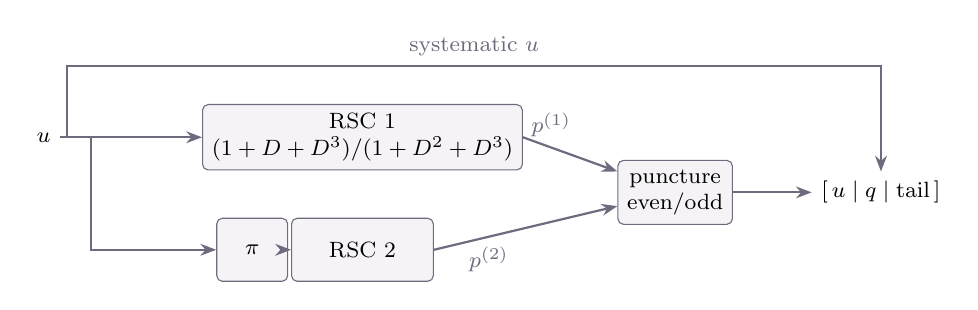
\begin{tikzpicture}[node distance=6mm and 10mm, every node/.style={font=\footnotesize},
  blk/.style={draw=icegrey, fill=iceground, rounded corners=2pt, align=center, minimum height=8mm, minimum width=18mm},
  arr/.style={-{Stealth[length=2mm]}, icegrey, thick}]
\node (u) {$u$};
\node[blk, right=18mm of u] (e1) {RSC 1\\$(1+D+D^3)/(1+D^2+D^3)$};
\node[blk, below=of e1, xshift=-14mm, minimum width=9mm] (pi) {$\pi$};
\node[blk, below=of e1] (e2) {RSC 2};
\coordinate (e2in) at (e2.west);
\node[blk, right=12mm of e1, yshift=-7mm, minimum width=14mm] (punc) {puncture\\even/odd};
\node[right=10mm of punc] (out) {$[\,u \mid q \mid \text{tail}\,]$};
\draw[arr] (u) -- (e1);
\draw[arr] ($(u)+(0.6,0)$) |- (pi.west);
\draw[arr] (pi) -- (e2);
\draw[arr] (e1.east) -- node[above,pos=0.3] {$p^{(1)}$} (punc);
\draw[arr] (e2.east) -- node[below,pos=0.3] {$p^{(2)}$} (punc);
\draw[arr] (punc) -- (out);
\draw[arr] ($(u)+(0.3,0)$) -- ++(0,0.9) -| node[above,pos=0.25] {systematic $u$} (out.north);
\end{tikzpicture}
\caption{Turbo encoder at rate $1/2$ (tail bits not drawn).}
\label{fig:turbo}
\end{figure}

\paragraph{Interleaver.}
The interleaver must exist for any message length $k$, from a few characters to an image, and be reproduced identically by the page and the script. It is built in three steps.
\begin{enumerate}
\item A 32-bit xorshift generator~\cite{marsaglia} is seeded with $x_0 = (\text{0x9E3779B9} \oplus k) \bmod 2^{32}$ (1 if that is 0); each step applies $x \leftarrow x \oplus (x \ll 13)$, $x \leftarrow x \oplus (x \gg 17)$, $x \leftarrow x \oplus (x \ll 5)$.
\item A Fisher--Yates shuffle~\cite{durstenfeld,knuth} of $(0, 1, \dots, k-1)$: for $i = k-1$ down to 1, draw the next $x$ and swap positions $i$ and $x \bmod (i+1)$.
\item A spreading pass (S-random interleaver~\cite{dolinar}) with $S = \min\bigl(16, \lfloor \sqrt{k/2} \rfloor\bigr)$: for $i = 0, 1, \dots$, look for the first $m \ge i$ such that $|\pi(m) - \pi(j)| > S$ for the $S$ previous positions $j = i-S, \dots, i-1$, and swap positions $i$ and $m$ (if there is none, position $i$ is left as it is).
\end{enumerate}
The spreading keeps message bits that are close together far apart after interleaving, which makes low-weight codewords rare (an input pattern that terminates one RSC encoder quickly is unlikely to terminate the other). The bound $S < \sqrt{k/2}$ is the usual condition for the construction to succeed~\cite{dolinar}. At $k = 456$ this interleaver performed as well as LTE's quadratic permutation polynomial interleaver in simulation.

\paragraph{Iterative decoding.}
Inside the turbo decoder, L-values follow the convention $\Lambda = \ln \frac{P(u=0)}{P(u=1)} = -\lambda$, clipped to $|\Lambda| \le 30$ for numerical safety (and to $\ell$ as in \cref{eq:viterbi}). Each constituent decoder is a log-MAP (BCJR) decoder~\cite{bcjr,robertson} on the 8-state trellis. For a transition from state $s$ with input $u$ and parities $p$, $p'$ at step $t$, with systematic L-value $\Lambda^{\mathrm s}_t$, a-priori L-value $\Lambda^{\mathrm a}_t$ and parity L-values $\Lambda^{\mathrm p}_t$, $\Lambda^{\mathrm p'}_t$ (zero where that parity is not sent, so $\Lambda^{\mathrm p'} = 0$ except at rate $1/4$), the branch metric is
\begin{equation}
\gamma_t(s, u) = \tfrac12 \bigl(\Lambda^{\mathrm s}_t + \Lambda^{\mathrm a}_t\bigr)(1 - 2u) + \tfrac12\, \Lambda^{\mathrm p}_t\, (1 - 2p) + \tfrac12\, \Lambda^{\mathrm p'}_t\, (1 - 2p').
\end{equation}
With the Jacobian logarithm $\maxstar(x, y) = \ln(e^x + e^y) = \max(x,y) + \ln\bigl(1 + e^{-|x-y|}\bigr)$, the forward and backward recursions are
\begin{align}
A_{t+1}(s') &= \maxstar_{(s,u) \to s'} \bigl[A_t(s) + \gamma_t(s,u)\bigr], & A_0(s) &= \begin{cases}0 & s = 0\\ -\infty & s \ne 0\end{cases},\\
B_t(s) &= \maxstar_{u} \bigl[\gamma_t(s,u) + B_{t+1}(s'(s,u))\bigr], & B_T(s) &= \begin{cases}0 & s = 0\\ -\infty & s \ne 0\end{cases},
\end{align}
both normalised at each step by subtracting their maximum, and the a-posteriori L-value of $u_t$ is
\begin{equation}
\Lambda_t = \maxstar_{(s,u):\,u=0} \bigl[A_t(s) + \gamma_t(s,u) + B_{t+1}(s')\bigr] - \maxstar_{(s,u):\,u=1} \bigl[A_t(s) + \gamma_t(s,u) + B_{t+1}(s')\bigr].
\end{equation}
The two decoders exchange \emph{extrinsic} information~\cite{hagenauer96}, what each learnt beyond its own inputs:
\begin{align}
\Lambda^{\mathrm e}_{1} &= \Lambda_{1} - \Lambda^{\mathrm s} - \Lambda^{\mathrm a}_{1}, \qquad \Lambda^{\mathrm a}_{1} = \Lambda^{\mathrm e}_{2} \text{ (de-interleaved)},\\
\Lambda^{\mathrm e}_{2} &= \Lambda_{2} - \Lambda^{\mathrm s}_{\pi} - \Lambda^{\mathrm a}_{2}, \qquad \Lambda^{\mathrm a}_{2} = \Lambda^{\mathrm e}_{1} \text{ (interleaved)},
\end{align}
where at rate $1/2$ decoder 1 uses the even parities and its own tail, and decoder 2 the interleaved systematic values, the odd parities and its own tail; at rates $1/3$ and $1/4$ each decoder gets its whole parity stream $p$, and at rate $1/4$ also its half of $q'$. After each iteration the decisions are $\hat u_{\pi(i)} = [\Lambda_{2,i} < 0]$; the decoder stops after 8 iterations, or earlier when the decisions no longer change from one iteration to the next (the page shows the number of iterations). Unlike the Viterbi algorithm, log-MAP decoding uses the size of the L-values, so it needs a well-scaled soft input (\cref{sec:alpha}).

\paragraph{Gain.}
On the textbook channel (BPSK, white Gaussian noise, 456 message bits) the turbo code needs about $1.3\dB$ less $E_b/N_0$ than the convolutional code for the same frame error rate (an LDPC code of the same length, tried for comparison, about $1.1\dB$). In the simulated rooms the gain shrinks to $0.5$--$1\dB$, roughly 10\,\% more distance: the bit error rate climbs steeply with distance, frames that fail have 15--19\,\% wrong channel bits, beyond what any rate-$1/2$ code corrects, and about $1\dB$ farther the frame itself is no longer detected.
On the textbook channel, rates $1/3$ and $1/4$ need $0.7$ and $1\dB$ less $E_b/N_0$ than rate $1/2$ (10\,\% frame errors at $1.4$, $0.7$ and $0.4\dB$, against $2.7\dB$ for the convolutional code; 400 frames per point). In the rooms they buy range only with airtime (\cref{tab:rates}).

\subsection{Reed--Solomon (255,223), received only}
\label{sec:rs}
Version~0 could send a Reed--Solomon code~\cite{reedsolomon}, and version~1 still decodes it.
\begin{itemize}
\item \emph{Field}: GF($2^8$) generated by the primitive polynomial $x^8 + x^4 + x^3 + x^2 + 1$ (0x11D), with primitive element $\alpha = x$.
\item \emph{Code}: generator $g(x) = \prod_{i=0}^{31} (x - \alpha^i)$; systematic codewords $c(x) = x^{32} m(x) + \bigl[x^{32} m(x) \bmod g(x)\bigr]$, minimum distance 33, correcting up to $t = 16$ wrong bytes per codeword.
\item \emph{Layout}: the $K = \lceil \nz/8 \rceil$ message bytes are split into $B = \lceil K/223 \rceil$ shortened codewords of nearly equal length, and the bytes of the codewords are sent interleaved (byte $j$ of each codeword in turn), so that a burst is shared between codewords.
\item \emph{Decoding}~\cite{berlekamp,massey,chien,forneybch}: hard decisions; syndromes $S_j = r(\alpha^j)$, $j = 0, \dots, 31$; the Berlekamp--Massey algorithm finds the error-locator polynomial $\Lambda(x)$; a Chien search finds its roots $X_\ell^{-1}$; Forney's formula gives the error values $e_\ell = X_\ell\, \Omega(X_\ell^{-1}) / \Lambda'(X_\ell^{-1})$ with $\Omega(x) = S(x)\Lambda(x) \bmod x^{32}$. A codeword is declared a failure if the number of roots differs from $\deg \Lambda$ or if the corrected word still has a non-zero syndrome.
\end{itemize}
\paragraph{Why it is no longer sent.}
In a room, Reed--Solomon fails as early as Hamming: both decide each bit before decoding and fail once about 1--2\,\% of the channel bits are wrong, while the convolutional and turbo decoders work on the soft values and still read texts with 5--9\,\% of the channel bits wrong (\cref{tab:rs}). Its advantage, a high rate, does not compensate. The header is unchanged (code 3 stays Reed--Solomon): giving code 3 to the turbo code would make version~0 receivers decode turbo frames as Reed--Solomon and show garbage instead of ignoring them.

The QR code that the page draws for the phones' link uses the same field and the same kind of Reed--Solomon code, with fewer parity bytes (byte mode, error-correction level M, versions 1--9~\cite{qr}).

%======================================================================
\section{Receiver}
\label{sec:rx}
The receiver needs no settings: the preamble length, the code, the rate, the tones and (version~2) the number of tones are all read from the frame. The page processes the microphone's samples as they arrive and fills in the message bit by bit; the script processes a whole recording.

\subsection{Non-coherent tone detectors}
\label{sec:energy}
For a tone $f$ and a window of $W$ samples starting at sample $m$, the detector output is the magnitude of one DFT coefficient,
\begin{equation}
E_f(m) = \Bigl| \sum_{n=0}^{W-1} y[m+n]\, e^{-j 2\pi f (m+n)/\fs} \Bigr| ,
\label{eq:energy}
\end{equation}
the envelope of a filter matched to a tone burst of unknown phase, i.e.\ the optimal non-coherent FSK detector~\cite{proakis}. It is computed at every sample by a running sum: with the prefix sums $S_f(n) = \sum_{\nu < n} y[\nu]\, e^{-j2\pi f\nu/\fs}$, $E_f(m) = |S_f(m+W) - S_f(m)|$, at a cost of one complex multiply--add per sample and tone. (The page keeps the last $W$ prefix sums in a ring buffer. For the 32 tones of the hopping control part it advances each phasor by a complex rotation and recomputes it exactly every 1024 samples, so that rounding errors do not accumulate.)

For the message part with hopping, the energies are computed only where they are needed: for symbol $k$, at the two tones of pair $p(k)$, with precomputed tables of $\cos$ and $\sin$.

\subsection{Frame detection}
\label{sec:detect}
\paragraph{Contrast.}
The detector works on the \emph{contrast} of the two control tones,
\begin{equation}
d(m) = \frac{E_1(m) - E_0(m)}{E_1(m) + E_0(m)} \in [-1, 1],
\end{equation}
which does not depend on the received level: the detector needs no automatic gain control and no noise estimate, and works the same for a phone next to the speaker and one at the back of the room.

\paragraph{Correlators.}
For each preamble length $N \in \{127, 255, 511\}$, with $a_j = 2P_j - 1$ the antipodal preamble and $o_j = \round{j \fs / \Rc}$ the offset of its bit $j$,
\begin{equation}
c_N(m) = \frac1N \sum_{j=0}^{N-1} a_j\, d(m + o_j), \qquad
c^{\mathrm{hop}}_N(m) = \frac1N \sum_{j=0}^{N-1} a_j\, d_{p(j)}(m + o_j),
\end{equation}
where $d_p$ is the contrast of hopping pair $p$ at 400 bit/s. The six correlators run side by side, and the frame is declared at the first local maximum of the score
\begin{equation}
\sigma(m) = \max_{\text{6 correlators}} \frac{c(m)}{\theta_N}, \qquad \theta_N = 0.3\sqrt{\frac{127}{N}},
\end{equation}
that exceeds 1. The winning correlator gives the preamble length and whether the control part hops.

\paragraph{Threshold.}
In noise alone, $E_0$ and $E_1$ are independent Rayleigh variables, so $d$ has zero mean and, by simulation, standard deviation $\sigma_d \approx 0.376$. The windows at the offsets $o_j$ do not overlap, so the terms of $c_N$ are independent and $c_N$ has standard deviation $\sigma_d/\sqrt N$. The threshold $\theta_N$ is $0.3\sqrt{127}/\sigma_d \approx 9.0$ standard deviations for every $N$: the three lengths have the same, very low, false-alarm rate. A longer preamble lowers the threshold by $\sqrt 2$ per doubling. When the SNR is low, the mean contrast is proportional to the SNR, so each doubling of $N$ lets the frame be found with about $1.5\dB$ less SNR (up to $3\dB$ at higher SNR). In simulation, the 511-bit preamble found every frame and read every header 2 to $4\dB$ below where the 127-bit preamble started missing them. No false detection occurred in 120\,s of noise, whistles and clicks.

\paragraph{Search.}
The correlation peak is about $2W$ samples wide, so the search advances in steps of $\max(2, \lfloor W/12 \rfloor)$ samples. When the score exceeds $0.85$, it steps back and scans sample by sample over the next $2W$ samples. If the best score there exceeds 1, the frame starts at its position $p_1$; otherwise the search resumes.

\subsection{Symbol timing: early--late gate}
\label{sec:track}
Symbol $k$ is read at $m_k = \round{\tau_k}$, where the real-valued instant $\tau_k$ advances by one symbol, $L_k = \fs/\Rc$ in the control part and $\fs/R$ in the message part. In between, an early--late gate~\cite{proakis,mengali} nudges it towards the instant where the tones are most distinct:
\begin{equation}
\tau_{k+1} = \tau_k + L_k + \mu\,\delta\,\bigl( |d(m_k + \delta)| - |d(m_k - \delta)| \bigr), \qquad \delta = \max\bigl(1, \round{W/4}\bigr), \quad \mu = 0.05 .
\end{equation}
If the window is late, the earlier window overlaps the symbol better, $|d(m_k - \delta)| > |d(m_k + \delta)|$, and $\tau$ moves earlier. The correction is skipped at $k = 0$ and at the first message symbol, where the window length changes. With hopping, the contrasts at $m_k \pm \delta$ are computed on the symbol's own pair. The small gain $\mu$ averages the correction over about 20 symbols. The tracking lets the page show the message correctly while it arrives; the final decisions use the instants of \cref{sec:clock}.

\subsection{Header decoding}
\label{sec:hdrdec}
For the 92 coded header bits the receiver uses the plain ratio $\ln(E_1/E_0)$ (with hopping, after levelling each tone over the preamble and header as in \cref{sec:level}). The $r$ copies are added, $\Lambda_i = \sum_{c=1}^{r} \ln(E_1/E_0)_{i,c}$, then Viterbi-decoded ($\ell = 4$), and the CRC and the fields are checked. Adding $r$ copies multiplies the signal part of the soft value by $r$ and its noise standard deviation by $\sqrt r$: a gain of $10\log_{10} r$ dB, 3 or $6\dB$ for 2 or 4 copies. An unreadable header sends the receiver back to the search, $W$ samples after $p_1$.

\subsection{Postamble and clock offset}
\label{sec:clock}
The two devices' sample clocks differ by tens to hundreds of parts per million (ppm); over a 20\,s frame, 100\,ppm is 2\,ms, more than a symbol at 1600 bit/s. The postamble measures this offset. In receiver samples, the nominal distance from the preamble to the postamble is
\begin{equation}
\Delta = (\NP + \NH)\frac{\fs}{\Rc} + \nc\, \frac{\fs}{R}, \qquad \NH = 92r ,
\end{equation}
and the postamble is searched within $\pm\round{3 \cdot 10^{-4}\,\Delta + L_R/4}$ samples of $p_1 + \Delta$ (clocks within $\pm 300$\,ppm, plus a quarter of a symbol), with the preamble correlator at the message's rate and tones. With hopping, it is searched first within $\pm 2$ symbols of where the tracking expects it (inside that window), then over the whole window. Version~1 searches within $\pm\bigl(\round{0.005\Delta} + \round{\fs/R}\bigr)$ samples (clocks within $\pm 5000$\,ppm), and with hopping first within $\pm 2$ symbols of the tracked position, inside the window or not. It is declared found if its correlation $c(p_2)$ is at least half that of the preamble, $c(p_1)$ (a fifth at 6400 bit/s, \cref{sec:wide}). Then
\begin{equation}
\rho = \frac{p_2 - p_1}{\Delta}, \qquad \text{clock offset} = (\rho - 1) \times 10^6\ \text{ppm},
\end{equation}
and the message and postamble energies are read again at the corrected instants
\begin{equation}
t_j = p_1 + \Bigl( (\NP + \NH)\frac{\fs}{\Rc} + j \frac{\fs}{R} \Bigr)\rho, \quad j = 0, \dots, \nc - 1, \qquad
t'_j = p_2 + j \frac{\fs}{R}\rho, \quad j = 0, \dots, \NP - 1 .
\end{equation}
If the postamble is not found (for instance when the end of the sound was cut off), the receiver keeps the instants of the early--late gate and estimates the soft output on the message itself (\cref{sec:em}).

\paragraph{Why 300\,ppm (version~2).}
The crystal clocks of audio hardware are usually within $\pm 50$\,ppm of their nominal rate, so two devices differ by about 100\,ppm at most, and $\pm 300$\,ppm leaves a wide margin. The wider window of version~1 cost nothing in a quiet room, but in strong echo the correlation with the postamble's known symbols can peak a symbol or more after the true postamble. The search then took that peak for a clock offset of 1000 to 4300\,ppm, and the message, re-read at the instants of that clock, was lost. With four tones at 400 bit/s and DRR $-14.6\dB$, the narrower window raised the texts read from 7 to 12 of 12 with the page's receiver and from 5 to 11 with the script's. Binary frames decoded as with version~1 in the other tests. The search of a room sounding's postamble (\cref{sec:sounding}) is unchanged.

\subsection{Tone levelling (hopping)}
\label{sec:level}
The speaker, the room and the microphone give each of the $2H$ tones its own level (on the real recording, the $1.6\kHz$ tone of the first band arrived about $10\dB$ weaker than the tones above $4.8\kHz$). Each tone's energies are divided by their root mean square over the symbols that used its pair,
\begin{equation}
\tilde E_{b,k} = \frac{E_{b,k}}{g_{b,p(k)}}, \qquad g_{b,p} = \sqrt{\frac{1}{|\mathcal K_p|} \sum_{k \in \mathcal K_p} E_{b,k}^2}, \qquad \mathcal K_p = \{k : p(k) = p\},
\end{equation}
over the message and the postamble together. Thanks to the scrambler, each tone carries the bit in about half of these symbols and only noise and echo in the others, so $g_{b,p}^2 \approx \tfrac12 A_{b,p}^2 + 2\sigma_{b,p}^2$ is the same mixture for every tone, and a single model (\cref{sec:llr}) then fits all of them. The page reports the spread $20\log_{10}(\max g / \min g)$ of the tone levels.

\subsection{Fine timing on the message (hopping)}
\label{sec:finetiming}
The instants $t_j$ come from the 400 bit/s preamble and the postamble. The preamble's long symbols tolerate a timing error of several samples (its correlation is flat within a few samples), the short symbols of a fast message do not: in the real 1600 bit/s recording the best instant was about 8 samples ($0.17\ms$, a quarter of a symbol) earlier. Once the whole message is in, the receiver therefore refines the timing on the message itself.
\begin{enumerate}
\item Cut the message into $K = \max\bigl(1, \min(8, \lfloor \nc/128 \rfloor)\bigr)$ blocks.
\item In each block, find the shift $\epsilon$, $|\epsilon| \le \epsilon_{\max} = \min\bigl(\lfloor \fs/(2R) \rfloor, \round{0.5\ms \cdot \fs}\bigr)$, that maximises the mean contrast $\overline{|E_1 - E_0|/(E_1 + E_0)}$ of the block's symbols read at $t_j + \epsilon$: on a grid of $\max(1, \round{\epsilon_{\max}/6})$ samples, then sample by sample around the best.
\item Fit a straight line through the $K$ points (block centre, best shift) by least squares; the line also absorbs a residual clock drift. Symbol $j$ is read at $t_j + \epsilon(j)$, with $\epsilon(j)$ the rounded value of the line, clipped to $\pm 2\epsilon_{\max}$.
\item Keep the new instants only if they make the tones clearly more distinct, symbol by symbol, than the instants used so far: with $\Delta_j$ the difference of the two contrasts at symbol $j$, a paired $t$-test requires $\bar\Delta > 2\, s_\Delta / \sqrt{\nc}$.
\end{enumerate}
This is done with hopping only. With fixed tones, the echo of the earlier bits lies on the same two tones, and in simulated rooms the contrast then often favoured a worse instant (at 1600 bit/s and DRR $0\dB$, 4 texts out of 6 were read instead of 6). With hopping, the echo lands on other pairs.

\subsection{Soft output}
\label{sec:soft}
The receiver offers two soft outputs, chosen on the receiver; switching after a reception re-decodes the same recording.

\paragraph{Plain ratio.}
$\lambda^{\mathrm{ratio}} = \ln\bigl((E_1 + \epsilon)/(E_0 + \epsilon)\bigr)$, $\epsilon = 10^{-9}$. It has the right sign when both tones arrive equally strong, but its size is not a reliability: it is the same for $(E_0, E_1) = (1, 2)$ and $(100, 200)$.

\paragraph{Calibrated LLR (default).}
\label{sec:llr}
Model the detector output of a tone as $Z = A e^{j\varphi} + N$, with an unknown phase $\varphi$ and complex Gaussian noise of variance $\sigma^2$ per real dimension. Its envelope $E = |Z|$ is Rician when the tone is sent and Rayleigh when it is not~\cite{rice,proakis}:
\begin{equation}
p_{\text{on}}(E) = \frac{E}{\sigma^2}\, e^{-\frac{E^2 + A^2}{2\sigma^2}}\, I_0\!\Bigl(\frac{AE}{\sigma^2}\Bigr), \qquad
p_{\text{off}}(E) = \frac{E}{\sigma^2}\, e^{-\frac{E^2}{2\sigma^2}},
\end{equation}
with $I_0$ the modified Bessel function of order 0. With the two tones independent given the bit (they are orthogonal), and tone $b$ having its own level $A_b$ and noise $\sigma_b^2$,
\begin{equation}
\lambda = \ln \frac{p_{\text{on},1}(E_1)\, p_{\text{off},0}(E_0)}{p_{\text{off},1}(E_1)\, p_{\text{on},0}(E_0)}
= \ln I_0\!\Bigl(\frac{A_1 E_1}{\sigma_1^2}\Bigr) - \frac{A_1^2}{2\sigma_1^2} - \ln I_0\!\Bigl(\frac{A_0 E_0}{\sigma_0^2}\Bigr) + \frac{A_0^2}{2\sigma_0^2} .
\label{eq:llr}
\end{equation}
Two limits help the intuition. At high SNR, $\ln I_0(x) \approx x - \tfrac12 \ln(2\pi x)$ and $\lambda$ is nearly linear in the envelopes, $\lambda \approx A_1 E_1/\sigma_1^2 - A_0 E_0/\sigma_0^2 + \dots$; at low SNR, $\ln I_0(x) \approx x^2/4$ and $\lambda$ compares the squared envelopes, the classical energy (square-law) detector. Unlike the ratio, \cref{eq:llr} corrects an imbalance between the tones and gives the decoders reliabilities on the right scale.

\paragraph{Calibration on the postamble.}
Since $\E[E^2] = A^2 + 2\sigma^2$ when the tone is on and $2\sigma^2$ when it is off, the receiver estimates, for each tone $b$, from the postamble's known bits,
\begin{equation}
P_{\text{on},b} = \overline{E_b^2}\big|_{P_j = b}, \quad P_{\text{off},b} = \overline{E_b^2}\big|_{P_j \neq b}, \qquad
\hat\sigma_b^2 = \frac{P_{\text{off},b}}{2}, \quad \hat A_b^2 = \max\bigl(P_{\text{on},b} - P_{\text{off},b},\ 10^{-6} P_{\text{on},b}\bigr).
\label{eq:cal}
\end{equation}
The postamble is used rather than the preamble because it is sent at the message's tones and rate. The page shows the SNR per symbol of each tone, $\hat A_b^2/(2\hat\sigma_b^2)$, which equals $E_s/N_0$: for a burst of amplitude $a$ over $W$ samples in white noise of variance $N_0/2$ per sample, $A = aW/2$ and $\sigma^2 = WN_0/4$.

$\ln I_0$ is evaluated with the polynomial approximations 9.8.1 ($x < 3.75$) and 9.8.2 ($x \ge 3.75$, in the form $x - \tfrac12 \ln x + \ln(\cdot)$) of Abramowitz and Stegun~\cite{abramowitz}, accurate to about $2 \times 10^{-7}$ relative.

\paragraph{Level tracking.}
In a room, most of the disturbance is the echo of the signal itself, so it rises and falls with the signal (someone walks between the speaker and the phone, the phone is moved). The receiver divides the energies by the local signal level relative to the calibration segment,
\begin{equation}
g_j = \sqrt{\clip\Bigl( \frac{1}{|\mathcal W_j|}\sum_{i \in \mathcal W_j} \frac{q_i}{\bar q_{\mathrm{ref}}},\ 0.01,\ 4 \Bigr)}, \qquad
q_i = \max\Bigl(\frac{E_{0,i}^2}{\hat A_0^2}, \frac{E_{1,i}^2}{\hat A_1^2}\Bigr), \qquad \mathcal W_j = \{i : |i - j| \le 24\},
\end{equation}
where $\bar q_{\mathrm{ref}}$ is the mean of $q$ over the postamble (over the message when the postamble is missing), and evaluates \cref{eq:llr} with $E_{b,j}/g_j$. The window of $\pm 24$ symbols averages out the bits while following slow changes; the clipping keeps $g_j$ within $[0.1, 2]$. This is right when echo dominates; if stationary noise dominated, dividing by $g$ would slightly misstate the reliabilities of the weak symbols.

\paragraph{Fitted scale.}
\label{sec:alpha}
The model assumes Gaussian noise. The echoes of short symbols have heavier tails, and on the real recording, even when calibrated on the true bits, the LLRs of \cref{eq:llr} were about 3 times too large. When the postamble is found, the LLR is multiplied by the factor $\alpha \le 1$ that best predicts the postamble's own bits under the logistic model $P(b_j = 1) = 1/(1 + e^{-\alpha\lambda_j})$:
\begin{equation}
\hat\alpha = \arg\max_{\alpha \in \mathcal A} \sum_{j=0}^{\NP - 1} -\ln\bigl(1 + e^{-\alpha\, a_j \lambda_j}\bigr), \qquad \mathcal A = \bigl\{0.05^{k/39} : k = 0, \dots, 39\bigr\},
\label{eq:alpha}
\end{equation}
a one-parameter version of Platt's logistic calibration~\cite{platt}. Since $\hat I(\alpha) = 1 - \frac{1}{\NP}\sum_j \log_2\bigl(1 + e^{-\alpha a_j \lambda_j}\bigr)$ is the usual estimate of the mutual information carried by the soft values~\cite{hagenauerexit}, $\hat\alpha$ also maximises that estimate. On the recording, a postamble emulated on 255 known message bits gave $\alpha \approx 0.3$, and the information per channel bit rose from 0.28--0.59 to 0.73--0.79 bit, the best any scale gives. In the model rooms $\alpha$ stays at 1. The scale matters for the turbo decoder, not for the Viterbi decoder (\cref{sec:conv}).

\paragraph{Blind calibration (postamble missing).}
\label{sec:em}
If the end of the sound was cut off (\cref{sec:txend}), there are no known bits. The receiver then estimates $A_b$ and $\sigma_b^2$ on the message itself, with an EM-style iteration~\cite{dempster}:
\begin{enumerate}
\item Start from the hard decisions, $w_j = [E_{1,j} > E_{0,j}]$, the probability that symbol $j$ carries a 1.
\item M-step: \cref{eq:cal} with every symbol weighted, $P_{\text{on},1} = \sum_j w_j E_{1,j}^2 / \sum_j w_j$, $P_{\text{off},1} = \sum_j (1-w_j) E_{1,j}^2 / \sum_j (1-w_j)$, and symmetrically for tone 0 with the weights $1 - w_j$ and $w_j$.
\item E-step: $w_j = 1/(1 + e^{-\lambda_j})$ with $\lambda_j$ from \cref{eq:llr}.
\item Repeat steps 2--3 (8 rounds in all).
\end{enumerate}
The E-step is exact under the model (with equally likely bits, which the scrambler ensures); the M-step uses the moment estimates instead of the exact maximum-likelihood ones, which keeps it simple and in closed form. There is no $\alpha$ in this case, and the LLRs stay somewhat too large.

\subsection{Decoding and the uncoded comparison}
\label{sec:decode}
The LLRs are descrambled, $\lambda_i \leftarrow (-1)^{k_i}\lambda_i$, de-interleaved and decoded (\cref{sec:codes}); the Viterbi and turbo decoders get $\ell = 4$ with the ratio and $\ell = \infty$ with the calibrated LLR. The receiver then re-encodes the decoded message, $\hat{\bm c} = \mathrm{Enc}(\hat{\bm u}) \oplus \bm k$, and counts the channel errors the code corrected, $\sum_i [\lambda_i > 0] \oplus \hat c_i$.

The page also shows what an uncoded frame would have shown with ``the same channel errors''. With $e_i = [\lambda_i > 0] \oplus \hat c_i$ the error pattern on the channel bits, it displays $\hat u_j \oplus e_j$ for $j = 0, \dots, \nz - 1$, the decoded message with the errors of the first $\nz$ channel positions applied. This assumes that the decoding was right and that the errors would fall the same way on an uncoded frame sent at the same channel bit rate (a binary symmetric channel; with hopping, the scrambler spreads each pair's errors evenly over both bits).

\subsection{Differences in the Python receiver}
\label{sec:pydiff}
\code{audiocomm\_v2.py} and \code{audiocomm\_v1.py} compute the same quantities on a whole recording with vectorised numpy code. They find the frame at the first sample where the score exceeds 1, then take the maximum over the next $2W$ samples. They have no early--late gate: without the postamble they read the symbols at the nominal instants ($\rho = 1$). Their fine timing compares the new instants with the unshifted instants $t_j$. Otherwise they decode the same frames to the same bits (checked on simulated recordings at every setting). For OFDM frames (version~3) the page and the script run the same steps and give the same clock offsets and the same corrected bits.

%======================================================================
\section{Room sounding}
\label{sec:sounding}
A room-sounding frame (header type 2) measures the impulse response $h$ of the whole chain, speaker, room and microphone, with a periodic maximum-length sequence~\cite{schroeder79,rife}.

\subsection{Excitation}
After the usual control part (the header gives the MLS order $m$ and the number of periods $P$), the transmitter plays an MLS of order $m \in \{14, 15, 16\}$, with feedback polynomials
\begin{equation}
x^{14} + x^{13} + x^{12} + x^{2} + 1, \qquad x^{15} + x^{14} + 1, \qquad x^{16} + x^{15} + x^{13} + x^{4} + 1,
\end{equation}
mapped to $\pm 0.35$ at $48\kHz$, one chip per sample. A period lasts $N = 2^m - 1$ samples: $0.34$, $0.68$ or $1.37$\,s. It is played $P+1$ times ($1 \le P \le 8$); the first period only fills the room, so that the following ones see the room in its periodic steady state. The postamble follows, in the control mode (4/8\,kHz, or hopping from its first bit). The sounding is heard as a loud hiss lasting $(P+1)N/\fsT$, from $0.7$ to $12.3$\,s; its rms level, $0.35$, is below that of the modem's tones ($0.9/\sqrt2 \approx 0.64$).

\paragraph{Choosing the period.}
The period must outlast the reverberation, otherwise the tail of the response folds back onto its start (time aliasing): $0.68$\,s suits a classroom, $1.37$\,s an amphitheatre.

\subsection{Impulse response}
Let $s_k = \pm 1$ be the MLS and $r_k$, $k = 0, \dots, N-1$, one received period, resampled to the transmitter's clock. In the steady state, $r$ is the circular convolution of $s$ with $h$ (if $h$ is shorter than $N$). By \cref{eq:mlsacf}, $\sum_k s_k s_{k-\tau} = (N+1)\delta_\tau - 1$, hence the circular cross-correlation
\begin{equation}
c_\tau = \sum_{k=0}^{N-1} r_k\, s_{(k-\tau) \bmod N} = (N+1)\, h_\tau - \sum_t h_t .
\end{equation}
An MLS has one more $+1$ than $-1$, so $\sum_k r_k = \sum_t h_t \sum_k s_k = \sum_t h_t$, and
\begin{equation}
h_\tau = \frac{c_\tau + \sum_k r_k}{N + 1} .
\label{eq:ir}
\end{equation}
The correlation is computed with a radix-2 FFT~\cite{cooleytukey} of length $2^{m+2}$ on two copies of the period. The $P$ periods are averaged before \cref{eq:ir}, which lowers the noise by $3\dB$ per doubling of $P$.

\subsection{Clock and glitches}
Each period must be resampled exactly to the transmitter's clock, or the averaged response is smeared.
\begin{enumerate}
\item The coarse ratio $\rho$ comes from the preamble--postamble distance, as in \cref{sec:clock}; it must be within $10^{-3}$ of 1 for the postamble to count as found.
\item The received signal is read at the fractional instants $t = t_{\text{first}} + (jN + k)\,\rho\,\fs/\fsT$ by Lanczos interpolation with $a = 6$, the kernel $\operatorname{sinc}(x)\operatorname{sinc}(x/6)$ over 12 samples~\cite{duchon}.
\item With $P \ge 2$, the position of the direct-path peak (refined by a parabola through the three largest samples) is measured in each period. Its least-squares slope over the periods, the drift in samples per period, refines the clock ratio: step $\times\,(1 + \text{drift}/N)$.
\item If the audio system dropped or repeated samples (a peak far from the fitted line, by more than one sample), each period is realigned on its own peak, the drift is taken as the median of the differences between consecutive peaks, and periods far from the median response are dropped (deviation above three times the median deviation; with two periods, the one with more energy around its peak is kept).
\end{enumerate}

\subsection{Post-processing}
The response is low-pass filtered (Blackman-windowed sinc, 97 taps, cut-off $\min(20\kHz, 0.45\fs)$), since the band above it only carries interpolation errors, and rotated so that the direct sound sits at $5\ms$. With $e_t = h_t^2$:
\begin{itemize}
\item \emph{Noise floor}: the mean of $e_t$ over the last 10\,\% of the period. \emph{End of the response} $t_{\text{end}}$: the first instant where $e$, smoothed over $\pm 2\ms$, falls below twice the floor.
\item \emph{Energy decay curve} (Schroeder backward integration~\cite{schroeder65}): $\mathrm{EDC}(t) = \sum_{t' = t}^{t_{\text{end}}} \max(0, e_{t'} - \text{floor}) + C$, in dB relative to $\mathrm{EDC}(0)$.
\item \emph{Reverberation time}: a straight line is fitted to the EDC in dB between $-5$ and $-25\dB$ ($T_{20}$) when the decay range above the noise is at least $35\dB$, else between $-5$ and $-15\dB$ ($T_{10}$) when it is at least $25\dB$~\cite{iso3382}; $T_{60} = -60/\text{slope}$. The decay hidden under the noise after $t_{\text{end}}$ is added back as the correction $C$, the value of the fitted line at $t_{\text{end}}$ (the backward integral of an exponential decay is the same exponential), and the fit is repeated twice, in the manner of Lundeby's method~\cite{lundeby}.
\item \emph{Direct-to-reverberant ratio}: $\mathrm{DRR} = 10\log_{10}\bigl(\sum_{|t - t_0| \le 2.5\ms} e_t \big/ (\text{rest, floor removed}, + C)\bigr)$, $t_0$ the direct sound. Beyond the critical distance it is negative and falls by about $6\dB$ per doubling of the distance~\cite{kuttruff}.
\item \emph{Clarity} $C_{50} = 10\log_{10}\bigl(\int_0^{50\ms} p^2 \big/ \int_{50\ms}^\infty p^2\bigr)$~\cite{iso3382}, floor removed, with the same correction.
\item \emph{RMS delay spread}: $\tau_{\mathrm{rms}} = \sqrt{\bar{t^2} - \bar t^{\,2}}$, the moments of the energy delay profile; the exponential tail beyond $t_{\text{end}}$ (time constant $\tau_s$) adds $C$, $C(t_e + \tau_s)$ and $C(t_e^2 + 2t_e\tau_s + 2\tau_s^2)$ to the moments of order 0, 1 and 2.
\item \emph{Frequency response}: $|H(f)|^2$ from an FFT of $h$ up to $t_{\text{end}}$, smoothed over $1/6$ octave on a grid of $1/24$ octave from $100\Hz$, and the gains at $4$, $8$ and $16\kHz$.
\item \emph{SNR per frequency}: Welch power spectra~\cite{welch} (Hann window, 2048 points, 50\,\% overlap) of the received sounding and of the noise heard before the frame (from $1.1$ to $0.15$\,s before the preamble), smoothed over $1/3$ octave: $\mathrm{SNR}(f) = 10\log_{10}\bigl((S(f) - N(f))/N(f)\bigr)$.
\end{itemize}
In simulation (rooms with $T_{60}$ from $0.4$ to $1.2$\,s and DRR from $-3$ to $+8\dB$, microphones at 44.1 and 48\,kHz, clock offsets up to $\pm 200$\,ppm), $T_{60}$, DRR, $C_{50}$ and $\tau_{\mathrm{rms}}$ came within 3\,\% (or $0.2\dB$) of the true response and the clock offset within 4\,ppm, also with 10\,ms of samples lost or repeated in the middle of the sounding.

\subsection{Room simulator (Python)}
\label{sec:roomsim}
\code{audiocomm\_v2.py sim} (or \code{audiocomm\_v1.py sim}) plays any frame through a measured response (\code{-{}-ir}) or through a model room: a direct sound at $5\ms$ plus a diffuse tail of Gaussian noise whose amplitude decays as $e^{-3\ln(10)\, t/T_{60}}$ (60\,dB of energy in $T_{60}$), faded in over $1$--$6\ms$, of length $5\ms + 1.5\,T_{60}$, and scaled so that its energy is $10^{-\mathrm{DRR}/10}$ times that of the direct sound. The output is then resampled to the microphone's rate with a clock offset (windowed-sinc resampling, 24 zero crossings, raised-cosine window, cut-off at $0.95$ of the lower Nyquist frequency), and white Gaussian noise is added at the requested SNR relative to the power of the received signal. This model has no early reflections; the simulations quoted in \cref{sec:params} also used a room model with early reflections and, where stated, the background noise of the real recording.

%======================================================================
\section{Transmitter timing}
\label{sec:txend}
Each \emph{Send} opens a fresh Web Audio context and plays the frame as one buffer at $48\kHz$. A long-lived context can end up suspended or interrupted (sleep, idle, change of output device) and then plays silence.

The context must not be closed as soon as the buffer has been handed over: the audio output still holds a few tenths of a second (more with Bluetooth). On the first real 1600 bit/s recording the sound stopped $0.2$\,s before the end of the frame, the postamble was lost, and the receiver calibrated its LLR on noise. The page now closes the context $2\,\text{s} + \text{outputLatency} + \text{baseLatency}$ after the end of playback, and the receiver handles a missing postamble (\cref{sec:em}). The postamble lasts $\NP/R$: with 255 bits, $0.16$\,s at 1600 bit/s but $1.3$\,s at 200 bit/s, which is why a short cut removed it entirely only at the highest rate.

%======================================================================
\section{Parameter choices}
\label{sec:params}
\Cref{tab:ptx,tab:prx,tab:psnd} list the parameters with the reason for each value. ``Simulation'' refers to the tests documented in \code{audioComm\_two\_devices.md}: model rooms ($T_{60} = 0.6$\,s unless stated, with early reflections), white noise or the background noise of the real recording, clock offsets and a 44.1\,kHz microphone, decoded by the page's receiver or the script.

\begin{table}[p]
\centering
\caption{Transmitter and frame.}
\label{tab:ptx}
\small
\begin{tabularx}{\linewidth}{>{\raggedright\arraybackslash}p{3.4cm}>{\raggedright\arraybackslash}p{3.1cm}X}
\toprule
Parameter & Value & Reason\\
\midrule
Sample rate & $48\kHz$ & Native rate of most audio hardware; every symbol is a whole number of samples ($L = 240, 120, 60, 30$).\\
Amplitude & $0.9$ & Loud, with a margin below full scale.\\
Bit rates $R$ & 200, 400, 800, 1600 bit/s & From robust (long symbols, more hopping pairs) to fast; at 1600 bit/s without hopping the room's echo dominates beyond short range.\\
Four tones (v2) & 2 bits per symbol, Gray mapping, tones $R/2$ apart & About $2\dB$ more tolerance of noise and 2--$3\dB$ of echo at the same bit rate, in the band of a binary pair (\cref{sec:mfsk}).\\
Four-tone rates & 400, 800, 1600, 3200, 6400 bit/s & The header's two rate bits, and tone set 3 for 6400 bit/s, the fastest FSK in the band (\cref{sec:wide}); 200 bit/s stays binary, and 3200 bit/s is too fast for binary FSK (timing tolerance, error floor).\\
Four-tone fixed sets & 4--8.8 or 8--12.8\,kHz, $1.6\kHz$ apart & Orthogonal at every rate; the low set stays where small speakers are good.\\
Fixed tones & $4/8\kHz$ (default), $8/16\kHz$ & 4 and 8\,kHz are well reproduced by phone and laptop speakers and microphones, and orthogonal at 200--800 bit/s. 8/16\,kHz were the original demo's tones; 16\,kHz is weak on phones and inaudible to some adults.\\
Control part & 400 bit/s, $4/8\kHz$ or hopping & A mode every receiver knows in advance; 400 bit/s is a compromise between robustness and the duration of the control part.\\
Warm-up & 40 bits (0.1\,s) & Lets the speaker's amplifier and the microphone's processing settle.\\
Silence & 0.2\,s before and after & Margin for the start and end of playback.\\
Preamble $\NP$ & 127 (default), 255, 511 & Longer preambles are found farther away (\cref{sec:detect}); 127 keeps short frames short.\\
Header copies $r$ & 1, 2, 4 & So that the header (3 or $6\dB$ gain) is read as far away as the longer preamble is found.\\
Header & 32 bits, CRC-8, conv.\ code & Self-describing frames with no settings on the receiver; the CRC rejects false detections.\\
Scrambler & $x^{15}+x^{14}+1$, seed all ones & Equal use of both tones whatever the message (needed by the calibration and the levelling); easy to reproduce in any language.\\
Interleaver & $\lceil\sqrt n\,\rceil$ columns & Spreads bursts as evenly as possible for any length.\\
Hopping band & 3.2 to 16\,kHz, $H = 6400/R$ & The width, 12.8\,kHz, gives $H = 32, 16, 8, 4$, powers of two as the pattern \cref{eq:hoppattern} requires; the start at 3.2\,kHz avoids the weak, noisy low tones (\cref{sec:hop}).\\
Hopping stride & $s = H/2 - 1$ & Visits every pair once per $H$ symbols; consecutive symbols about half the band apart.\\
Turbo code & LTE constituents, S-random & Same length as the convolutional code; the well-studied 8-state constituents of LTE; an interleaver defined for any length.\\
Turbo code rates & $1/2$, $1/3$, $1/4$, nested & Lower rates for the farthest phones, with the 511 preamble; in the same airtime a lower bit rate does as well in noise and better in echo (\cref{tab:rates}).\\
TX close delay & $2\,\text{s}$ + output latency & Lets the speaker play the end of the frame (\cref{sec:txend}).\\
OFDM band (v3) & 3.2 to 16\,kHz & The band of tone hopping: the weak, noisy low frequencies are avoided, and 16\,kHz is still reproduced by most phones and laptops.\\
OFDM guard (v3) & $21.3\ms$ ($N = 2048$) or $5.3\ms$ ($N = 1024$) & The long guard holds most of a classroom's early echo for a third of the airtime; the short one shows what happens when the echo outlasts the guard (\cref{sec:ofdmres}).\\
OFDM mapping (v3) & DQPSK, Gray & No estimate of the room's response is needed, and phase noise from a moving phone only matters between consecutive symbols (\cref{sec:dqpsk}).\\
OFDM level (v3) & rms 0.45, clipped at 0.9 & Half the FSK peak: $4.5\,\%$ of the samples are clipped, with the clipping noise $19\dB$ below the signal.\\
Reference symbol (v3) & Newman phases, sent first and last & Low peaks (never clipped); the pair gives the time scale (\cref{sec:ofdmrx}).\\
\bottomrule
\end{tabularx}
\end{table}

\begin{table}[p]
\centering
\caption{Receiver.}
\label{tab:prx}
\small
\begin{tabularx}{\linewidth}{>{\raggedright\arraybackslash}p{3.4cm}>{\raggedright\arraybackslash}p{3.1cm}X}
\toprule
Parameter & Value & Reason\\
\midrule
Microphone processing & echo cancellation, noise suppression and AGC off & They distort or remove tones; the contrast detector needs no AGC.\\
Detection window & one symbol, $W = \round{\fs/R}$ & The matched (integrate-and-dump) window of a rectangular burst.\\
Detection threshold & $\theta_N = 0.3\sqrt{127/N}$ & About 9 noise standard deviations for every preamble length (\cref{sec:detect}).\\
Search step & $\max(2, \lfloor W/12 \rfloor)$, then 1 & The peak is about $2W$ wide; a coarse step saves computation (the hopping receiver needs less computing than version~0's).\\
Candidate level & $0.85\,\theta_N$ & Starts the fine scan slightly before the threshold is reached.\\
Early--late gate & $\delta = W/4$, $\mu = 0.05$ & Quarter-symbol offsets are sensitive to timing yet inside the symbol; a small gain averages over about 20 symbols.\\
Postamble window & $\pm(300$\,ppm of $\Delta$ $+\ \tfrac14$ symbol$)$; v1: $\pm(0.5\,\%$ of $\Delta$ $+$ 1 symbol$)$ & Covers any realistic clock offset; in strong echo, v1's wider window let late correlation peaks pass for offsets of thousands of ppm (\cref{sec:clock}).\\
Postamble found & $c(p_2) \ge \tfrac12 c(p_1)$ & Accepts a postamble weakened by distance or echo, rejects noise.\\
Header soft value & $\ln(E_1/E_0)$, clipped at 4 & Needs no calibration (no known bits at the message's rate yet).\\
Calibration & Rician/Rayleigh moments on the postamble & Postamble sent at the message's tones and rate; closed-form estimates.\\
Level tracking & $\pm 24$ symbols, $g \in [0.1, 2]$ & Long enough to average the bits, short enough to follow movements.\\
Levelling, four tones & rms where the tone is the strongest & A tone is sent in only a quarter of its group's symbols (\cref{sec:mfskrx}).\\
Scale $\alpha$ & 40 values from 1 to 0.05 & Corrects over-confident LLRs (heavy-tailed echo); log-spaced grid.\\
Blind EM & 8 rounds & Converges in a few rounds from the hard decisions.\\
Fine timing & $K \le 8$ blocks of $\ge 128$ symbols, $|\epsilon| \le \min(T/2, 0.5\ms)$, $t > 2$ & Enough symbols per block for a stable contrast; the $t$-test keeps the old instants unless the new ones are clearly better.\\
Viterbi clipping $\ell$ & 4 (ratio), $\infty$ (calibrated) & Limits the weight of clicks with the uncalibrated ratio.\\
Turbo iterations & $\le 8$, early stop & Stops as soon as the decisions settle (3--4 iterations on the real recording), which saves time on phones.\\
OFDM interpolation (v3) & sinc, Hann window, $A = 16$ & Reads the recording on the transmitter's grid at any rate and time scale, with errors far below the noise.\\
OFDM timing (v3) & latest stretch with $\ge 99\,\%$ of the most energy & Puts the direct sound at the start of the guard, so that the guard covers as much later echo as possible.\\
OFDM time scale (v3) & $\pm 500$\,ppm, 1\,ppm steps, parabola & Covers clock offsets and a phone moving at up to about 0.17\,m/s; the phase error left is far below DQPSK's $45^\circ$.\\
OFDM window margin (v3) & 8 samples & Keeps the direct sound inside the guard if the timing is slightly late.\\
OFDM noise groups (v3) & 32 subcarriers & Enough decisions for a stable estimate of $N_0$, narrow enough to follow the room's response and the speaker's.\\
\bottomrule
\end{tabularx}
\end{table}

\begin{table}[ht]
\centering
\caption{Room sounding.}
\label{tab:psnd}
\small
\begin{tabularx}{\linewidth}{>{\raggedright\arraybackslash}p{3.4cm}>{\raggedright\arraybackslash}p{3.1cm}X}
\toprule
Parameter & Value & Reason\\
\midrule
MLS order & 14, 15 (default), 16 & Period 0.34, 0.68, 1.37\,s: must outlast the reverberation.\\
Periods & 1--8 (+1 to fill the room) & $3\dB$ less noise per doubling; longer soundings are tiresome.\\
Amplitude & $\pm 0.35$ & Quieter than the tones; a binary signal has crest factor 1, so it is still loud.\\
Interpolation & Lanczos, $a = 6$ & Band-limited resampling with a short kernel.\\
Low-pass & $\min(20\kHz, 0.45\fs)$ & Removes interpolation errors above the audio band.\\
$T_{20}$ / $T_{10}$ & decay range $\ge 35$ / $25\dB$ & Standard evaluation ranges~\cite{iso3382}, each with $10\dB$ of margin above the noise.\\
DRR window & $\pm 2.5\ms$ & Contains the direct sound, excludes most early reflections.\\
\bottomrule
\end{tabularx}
\end{table}

\subsection{Evidence from simulation and the real recording}
\label{sec:results}
The following tables, from \code{audioComm\_two\_devices.md}, motivated the main choices. They are simulations unless stated; the demo has been tried with one real recording so far (hopping, 1600 bit/s, turbo code, demo image), which now decodes with no pixel errors.

\begin{table}[ht]
\centering
\caption{Fixed tones against tone hopping (convolutional code, 57-character text, 8 trials per cell, texts read right). Measured with the earlier hopping band starting at $1.6\kHz$.}
\label{tab:plainhop}
\small
\begin{tabular}{lcccc}
\toprule
& \multicolumn{2}{c}{400 bit/s, preamble 127} & \multicolumn{2}{c}{200 bit/s, preamble 511}\\
\cmidrule(lr){2-3}\cmidrule(lr){4-5}
DRR & 4/8\,kHz & hopping & 4/8\,kHz & hopping\\
\midrule
$+3\dB$ & 8 & 8 & 8 & 8\\
$0\dB$ & 6 & 8 & 8 & 8\\
$-3\dB$ & 3 & 8 & 1 & 8\\
$-6\dB$ & 0 & 8 & 0 & 8\\
$-9\dB$ & 0 & 8 & 0 & 8\\
$-12\dB$ & 0 & 2 & 0 & 8\\
\bottomrule
\end{tabular}
\end{table}
With the textbook rule that the DRR falls by about $6\dB$ per doubling of the distance beyond the critical distance, \cref{tab:plainhop} moves the range from about $1.4$ times the critical distance (fixed tones) to about 3 times (hopping, 400 bit/s) or 4 times (hopping, 200 bit/s). This conversion is a rule of thumb, not a measurement. Beyond the critical distance, a longer preamble or a lower rate does not help fixed tones, whose limit is the room's own echo; with hopping, both help again.

\begin{table}[ht]
\centering
\caption{Codes far from the speaker (hopping, 400 bit/s, 57-character text, 24 trials with the same rooms and noise for each code, texts read right). LDPC was tried for comparison only.}
\label{tab:turbo}
\small
\begin{tabular}{lccc}
\toprule
Limited by & Convolutional & LDPC & Turbo\\
\midrule
echo, DRR $-11\dB$ & 21 & 23 & 22\\
echo, DRR $-12\dB$ & 14 & 17 & 18\\
echo, DRR $-13\dB$ & 4 & 6 & 7\\
noise, SNR $-9\dB$ & 14 & 22 & 22\\
noise, SNR $-10\dB$ & 2 & 12 & 14\\
\bottomrule
\end{tabular}
\end{table}

\begin{table}[ht]
\centering
\caption{Turbo code rates against bit rates (hopping, preamble 511, 57-character text, $T_{60} = 0.6$\,s, the page's receiver). Frame: the length of the sound. Noise: DRR $+6\dB$, white noise; the SNR over $3.2$--$16\kHz$ at which half of 12 texts are read ($^{\ast}$the frame detection fails first). Echo: little noise; texts read right out of 24 rooms. Rows with the same message bit rate use the same airtime. $^{\dagger}$Separate run: 1 of 12 texts at DRR $-12\dB$, against 8 of 12 for 400 bit/s at rate $1/2$.}
\label{tab:rates}
\small
\setlength{\tabcolsep}{4.5pt}
\begin{tabular}{ccccrccccccc}
\toprule
& & & & & \multicolumn{7}{c}{echo: texts read at DRR (dB)}\\
\cmidrule(lr){6-12}
bit/s & code rate & message bit/s & frame (s) & SNR (dB) & $-12$ & $-14$ & $-16$ & $-18$ & $-20$ & $-22$ & $-24$\\
\midrule
800 & $1/4$ & 200 & 5.6 & $-8.7$ & \multicolumn{7}{c}{see $^{\dagger}$}\\
400 & $1/2$ & 200 & 6.3 & $-9.0$ & 19 & 2 & 0 & 0 & 0 & 0 & 0\\
400 & $1/3$ & 133 & 7.4 & $-10.6$ & 22 & 16 & 2 & 1 & 3 & 1 & 1\\
400 & $1/4$ & 100 & 8.6 & $-11.7$ & 23 & 22 & 11 & 7 & 9 & 8 & 5\\
200 & $1/2$ & 100 & 9.9 & $-11.3$ & 24 & 22 & 13 & 16 & 16 & 16 & 17\\
200 & $1/3$ & 67 & 12.2 & $-12.4^{\ast}$ & 24 & 24 & 21 & 23 & 24 & 24 & 24\\
200 & $1/4$ & 50 & 14.5 & $-12.5^{\ast}$ & 24 & 24 & 24 & 24 & 24 & 24 & 24\\
\bottomrule
\end{tabular}
\end{table}

\paragraph{Code rate or bit rate?}
\Cref{tab:rates} compares lowering the turbo code's rate with lowering the bit rate. In noise, at a fixed bit rate, rates $1/3$ and $1/4$ tolerate $1.6$ and $2.7\dB$ more noise than rate $1/2$, but the frame lasts longer; spent on a lower bit rate, the same airtime does as well ($400$ bit/s at $1/4$ and $200$ bit/s at $1/2$ are $0.4\dB$ apart, $800$ bit/s at $1/4$ and $400$ bit/s at $1/2$ are $0.3\dB$ apart). The $1\dB$ that rate $1/4$ gains on the textbook channel is lost, probably to the non-coherent detector, which loses more when each channel bit carries less energy (the non-coherent combining loss~\cite{proakis}). In echo, far beyond the critical distance, the bit rate counts more: from DRR $-16$ to $-24\dB$, in the same airtime, $200$ bit/s at rate $1/2$ read 78 of 120 texts and $400$ bit/s at rate $1/4$ read 40. Below about $-16\dB$ the counts stop falling: the phone hears mostly reverberation, and the interference is the reverberation of the earlier symbols on the same tone pair. A pair is used again after $H$ symbols, $40\ms$ at 400 bit/s and $160\ms$ at 200 bit/s, by which time the reverberation has decayed by $4$ and $16\dB$; halving the bit rate doubles this wait, lowering the code rate does not change it, which probably explains the difference. Combined, 200 bit/s at rate $1/3$ or $1/4$ read 116 and 120 of these 120 texts. With the 127-bit preamble the frame itself is lost at about the noise and echo where rate $1/2$ already fails, so the lower rates need the 511-bit preamble.

\begin{table}[ht]
\centering
\caption{All five codes (57-character text, $T_{60} = 0.6$\,s, the real recording's noise, 6 trials per row, texts read right; $^{\ast}$5 of the 6 frames were found).}
\label{tab:rs}
\small
\begin{tabular}{lccccc}
\toprule
Setting & None & Hamming & RS & Conv. & Turbo\\
\midrule
hopping 400 bit/s, DRR $-6\dB$, SNR $20\dB$ & 2 & 6 & 6 & 6 & 6\\
hopping 400 bit/s, DRR $-9\dB$, SNR $20\dB$ & 0 & 1 & 1 & 6 & 6\\
hopping 400 bit/s, DRR $-12\dB$, SNR $20\dB$ & 0 & 0 & 0 & 2 & 3\\
hopping 400 bit/s, DRR $0\dB$, SNR $3\dB$ & 0 & 3 & 3 & 6 & 6\\
hopping 400 bit/s, DRR $0\dB$, SNR $0\dB$ & 0 & 0 & 0 & 6 & 6\\
hopping 1600 bit/s, DRR $0\dB$, SNR $6\dB$ & 0 & 1 & 4 & 6 & 6\\
4/8\,kHz 400 bit/s, DRR $0\dB$, SNR $20\dB$$^{\ast}$ & 0 & 1 & 3 & 5 & 5\\
\bottomrule
\end{tabular}
\end{table}

\begin{table}[ht]
\centering
\caption{Hopping band starting at $1.6\kHz$ (old) or $3.2\kHz$ (new), 1600 bit/s, texts read right out of 6. ``Rolled-off'': a speaker attenuating below $2.8\kHz$, like the real one.}
\label{tab:band}
\small
\begin{tabular}{lcc}
\toprule
Setting & Convolutional & Turbo\\
\midrule
flat speaker, DRR $0\dB$, SNR $3\dB$ & $2 \to 6$ & $5 \to 6$\\
flat speaker, DRR $0\dB$, SNR $0\dB$ & $1 \to 3$ & $1 \to 6$\\
rolled-off speaker, DRR $-3\dB$, SNR 16 / 12 / $9\dB$ & 4 / 3 / 2 $\to$ 6 / 4 / 5 & 5 / 5 / 4 $\to$ 6 / 6 / 5\\
flat speaker, DRR $-6\dB$, SNR 22 / 16 / $12\dB$ & 3 / 1 / 0 $\to$ 3 / 1 / 0 & 4 / 3 / 1 $\to$ 5 / 4 / 3\\
\bottomrule
\end{tabular}
\end{table}

\begin{table}[ht]
\centering
\caption{Two tones against four (version~2; tone hopping, turbo code rate $1/2$, preamble 511, 57-character text, $T_{60} = 0.6$\,s, 16 trials per point on a $1\dB$ grid, the script's receiver; on the same recordings, 12 per point, the page's receiver read the same number of texts within 1 or 2). Noise: DRR $+6\dB$, white noise, the SNR over $3.2$--$16\kHz$ at which half the texts are read. Echo: SNR $40\dB$, the DRR at which half, and 9 in 10, of the texts are read. Lower is better; the gains are in dB.}
\label{tab:mfsk}
\small
\begin{tabular}{rcccccc}
\toprule
& \multicolumn{3}{c}{noise: SNR (dB)} & \multicolumn{3}{c}{echo: DRR (dB), half / 9 in 10}\\
\cmidrule(lr){2-4}\cmidrule(lr){5-7}
bit/s & 2 tones & 4 tones & gain & 2 tones & 4 tones & gain\\
\midrule
400 & $-8.4$ & $-10.3$ & 1.9 & $-12.6$ / $-11.6$ & $-15.5$ / $-14.6$ & 2.9 / 3.0\\
800 & $-5.4$ & $-7.8$ & 2.4 & $-9.1$ / $-7.8$ & $-10.5$ / $-9.7$ & 1.4 / 1.9\\
1600 & $-2.5$ & $-4.5$ & 2.0 & $-7.0$ / above $-4.8$ & $-7.3$ / $-6.5$ & 0.3 / over 1.7\\
3200 & --- & $-1.7$ & & --- & $-5.2$ / $-3.5$ & \\
\bottomrule
\end{tabular}
\end{table}

\paragraph{Four tones or two?}
At the same bit rate, four tones tolerated about $2\dB$ more noise and, for 9 texts in 10, 2 to $3\dB$ more echo (\cref{tab:mfsk}). Half-way, the echo gain is smaller at 1600 bit/s ($0.3\dB$), where two tones fail gradually: 13 of 16 texts were still read $2\dB$ above their half-way point. With the rule of $6\dB$ per doubling of the distance (in the direct field for noise, beyond the critical distance for the DRR), 2 to $3\dB$ is 25 to 40\,\% more distance; this is a rule of thumb, not a measurement. Four tones at $2R$, twice the throughput, needed only $0.6$ to $0.9\dB$ more SNR than two tones at $R$, but about $2\dB$ more DRR: 3200 bit/s, with four tones only, needed $0.8\dB$ more SNR and $1.8\dB$ more DRR than binary at 1600 bit/s. The real receiver came within about $0.5\dB$ of the ideal receiver of the study in noise. In deep echo at 1600 and 3200 bit/s the four-tone postamble was often not found, and the texts were then read with the blind calibration of \cref{sec:em}.

\paragraph{The real recording.}
On the 1600 bit/s hopping recording, the improvements of version~1 were measured one by one: handling the missing postamble took the calibrated LLR from 1373 pixel errors to 0; fine timing and the fitted scale lowered the channel errors from $8.2$ to $6.1\,\%$ and the turbo iterations from 8 to 3--4; the per-pair error count then pointed to the lowest tone pair, which led to the $3.2\kHz$ band.

\paragraph{Not yet verified on real hardware.}
Room sounding, the new hopping band (top tones up to $15.8\kHz$ at 200 bit/s), long-range hopping, the turbo rates $1/3$ and $1/4$, the four tones of version~2 and the OFDM of version~3 have been tested in simulation and with the page in a browser fed simulated recordings, not yet with real phones in a real room. A classroom test with recordings saved from the phones would confirm them.

%======================================================================
\clearpage
\begin{thebibliography}{99}
\small

\bibitem{proakis}
J.~G. Proakis and M.~Salehi, \emph{Digital Communications}, 5th~ed. New York: McGraw-Hill, 2008.

\bibitem{lincostello}
S.~Lin and D.~J. Costello, \emph{Error Control Coding}, 2nd~ed. Upper Saddle River, NJ: Pearson Prentice Hall, 2004.

\bibitem{golomb}
S.~W. Golomb, \emph{Shift Register Sequences}. San Francisco: Holden-Day, 1967.

\bibitem{ieee80211}
\emph{IEEE Standard for Information Technology---Telecommunications and Information Exchange between Systems---Local and Metropolitan Area Networks---Specific Requirements, Part~11: Wireless LAN Medium Access Control (MAC) and Physical Layer (PHY) Specifications}, IEEE Std 802.11-2020.

\bibitem{petersonbrown}
W.~W. Peterson and D.~T. Brown, ``Cyclic codes for error detection,'' \emph{Proc. IRE}, vol.~49, no.~1, pp.~228--235, Jan. 1961.

\bibitem{itui432}
ITU-T Recommendation I.432.1, \emph{B-ISDN user-network interface---Physical layer specification: General characteristics}, 1999.

\bibitem{ts36212}
3GPP TS 36.212, \emph{Evolved Universal Terrestrial Radio Access (E-UTRA); Multiplexing and channel coding}.

\bibitem{cdma2000}
3GPP2 C.S0002, \emph{Physical Layer Standard for cdma2000 Spread Spectrum Systems}.

\bibitem{dvbs}
ETSI EN 300 421, \emph{Digital Video Broadcasting (DVB); Framing structure, channel coding and modulation for 11/12~GHz satellite services}, 1997.

\bibitem{kuttruff}
H.~Kuttruff, \emph{Room Acoustics}, 5th~ed. London: Spon Press, 2009.

\bibitem{kilfoyle}
D.~B. Kilfoyle and A.~B. Baggeroer, ``The state of the art in underwater acoustic telemetry,'' \emph{IEEE J. Oceanic Eng.}, vol.~25, no.~1, pp.~4--27, Jan. 2000.

\bibitem{whoi}
L.~Freitag, M.~Grund, S.~Singh, J.~Partan, P.~Koski, and K.~Ball, ``The WHOI Micro-Modem: an acoustic communications and navigation system for multiple platforms,'' in \emph{Proc. MTS/IEEE OCEANS}, 2005.

\bibitem{hamming}
R.~W. Hamming, ``Error detecting and error correcting codes,'' \emph{Bell Syst. Tech. J.}, vol.~29, no.~2, pp.~147--160, 1950.

\bibitem{viterbi}
A.~J. Viterbi, ``Error bounds for convolutional codes and an asymptotically optimum decoding algorithm,'' \emph{IEEE Trans. Inf. Theory}, vol.~13, no.~2, pp.~260--269, Apr. 1967.

\bibitem{forneyva}
G.~D. Forney, Jr., ``The Viterbi algorithm,'' \emph{Proc. IEEE}, vol.~61, no.~3, pp.~268--278, Mar. 1973.

\bibitem{berrou}
C.~Berrou, A.~Glavieux, and P.~Thitimajshima, ``Near Shannon limit error-correcting coding and decoding: Turbo-codes,'' in \emph{Proc. IEEE Int. Conf. Commun. (ICC)}, Geneva, 1993, pp.~1064--1070.

\bibitem{marsaglia}
G.~Marsaglia, ``Xorshift RNGs,'' \emph{J. Stat. Softw.}, vol.~8, no.~14, pp.~1--6, 2003.

\bibitem{durstenfeld}
R.~Durstenfeld, ``Algorithm 235: Random permutation,'' \emph{Commun. ACM}, vol.~7, no.~7, p.~420, 1964.

\bibitem{knuth}
D.~E. Knuth, \emph{The Art of Computer Programming, Vol.~2: Seminumerical Algorithms}, 3rd~ed. Reading, MA: Addison-Wesley, 1997, Sec.~3.4.2.

\bibitem{dolinar}
S.~Dolinar and D.~Divsalar, ``Weight distributions for turbo codes using random and nonrandom permutations,'' JPL TDA Progress Report 42-122, Aug. 1995.

\bibitem{bcjr}
L.~R. Bahl, J.~Cocke, F.~Jelinek, and J.~Raviv, ``Optimal decoding of linear codes for minimizing symbol error rate,'' \emph{IEEE Trans. Inf. Theory}, vol.~20, no.~2, pp.~284--287, Mar. 1974.

\bibitem{robertson}
P.~Robertson, E.~Villebrun, and P.~Hoeher, ``A comparison of optimal and sub-optimal MAP decoding algorithms operating in the log domain,'' in \emph{Proc. IEEE Int. Conf. Commun. (ICC)}, Seattle, 1995, pp.~1009--1013.

\bibitem{hagenauer96}
J.~Hagenauer, E.~Offer, and L.~Papke, ``Iterative decoding of binary block and convolutional codes,'' \emph{IEEE Trans. Inf. Theory}, vol.~42, no.~2, pp.~429--445, Mar. 1996.

\bibitem{reedsolomon}
I.~S. Reed and G.~Solomon, ``Polynomial codes over certain finite fields,'' \emph{J. SIAM}, vol.~8, no.~2, pp.~300--304, 1960.

\bibitem{berlekamp}
E.~R. Berlekamp, \emph{Algebraic Coding Theory}. New York: McGraw-Hill, 1968.

\bibitem{massey}
J.~L. Massey, ``Shift-register synthesis and BCH decoding,'' \emph{IEEE Trans. Inf. Theory}, vol.~15, no.~1, pp.~122--127, Jan. 1969.

\bibitem{chien}
R.~T. Chien, ``Cyclic decoding procedures for Bose--Chaudhuri--Hocquenghem codes,'' \emph{IEEE Trans. Inf. Theory}, vol.~10, no.~4, pp.~357--363, Oct. 1964.

\bibitem{forneybch}
G.~D. Forney, Jr., ``On decoding BCH codes,'' \emph{IEEE Trans. Inf. Theory}, vol.~11, no.~4, pp.~549--557, Oct. 1965.

\bibitem{qr}
ISO/IEC 18004:2015, \emph{Information technology---Automatic identification and data capture techniques---QR Code bar code symbology specification}.

\bibitem{mengali}
U.~Mengali and A.~N. D'Andrea, \emph{Synchronization Techniques for Digital Receivers}. New York: Plenum, 1997.

\bibitem{rice}
S.~O. Rice, ``Mathematical analysis of random noise,'' \emph{Bell Syst. Tech. J.}, vol.~23, pp.~282--332, 1944, and vol.~24, pp.~46--156, 1945.

\bibitem{abramowitz}
M.~Abramowitz and I.~A. Stegun, Eds., \emph{Handbook of Mathematical Functions}, NBS Applied Mathematics Series~55. Washington, DC, 1964, Sec.~9.8.

\bibitem{platt}
J.~C. Platt, ``Probabilistic outputs for support vector machines and comparisons to regularized likelihood methods,'' in \emph{Advances in Large Margin Classifiers}, A.~Smola, P.~Bartlett, B.~Sch\"olkopf, and D.~Schuurmans, Eds. Cambridge, MA: MIT Press, 2000, pp.~61--74.

\bibitem{hagenauerexit}
J.~Hagenauer, ``The EXIT chart: introduction to extrinsic information transfer in iterative processing,'' in \emph{Proc. European Signal Processing Conf. (EUSIPCO)}, Vienna, 2004.

\bibitem{dempster}
A.~P. Dempster, N.~M. Laird, and D.~B. Rubin, ``Maximum likelihood from incomplete data via the EM algorithm,'' \emph{J. R. Stat. Soc. B}, vol.~39, no.~1, pp.~1--38, 1977.

\bibitem{schroeder79}
M.~R. Schroeder, ``Integrated-impulse method measuring sound decay without using impulses,'' \emph{J. Acoust. Soc. Am.}, vol.~66, no.~2, pp.~497--500, 1979.

\bibitem{rife}
D.~D. Rife and J.~Vanderkooy, ``Transfer-function measurement with maximum-length sequences,'' \emph{J. Audio Eng. Soc.}, vol.~37, no.~6, pp.~419--444, 1989.

\bibitem{cooleytukey}
J.~W. Cooley and J.~W. Tukey, ``An algorithm for the machine calculation of complex Fourier series,'' \emph{Math. Comput.}, vol.~19, no.~90, pp.~297--301, 1965.

\bibitem{duchon}
C.~E. Duchon, ``Lanczos filtering in one and two dimensions,'' \emph{J. Appl. Meteorol.}, vol.~18, no.~8, pp.~1016--1022, 1979.

\bibitem{schroeder65}
M.~R. Schroeder, ``New method of measuring reverberation time,'' \emph{J. Acoust. Soc. Am.}, vol.~37, no.~3, pp.~409--412, 1965.

\bibitem{iso3382}
ISO 3382-1:2009, \emph{Acoustics---Measurement of room acoustic parameters---Part~1: Performance spaces}; ISO 3382-2:2008, \emph{Part~2: Reverberation time in ordinary rooms}.

\bibitem{lundeby}
A.~Lundeby, T.~E. Vigran, H.~Bietz, and M.~Vorl\"ander, ``Uncertainties of measurements in room acoustics,'' \emph{Acustica}, vol.~81, no.~4, pp.~344--355, 1995.

\bibitem{welch}
P.~D. Welch, ``The use of fast Fourier transform for the estimation of power spectra: a method based on time averaging over short, modified periodograms,'' \emph{IEEE Trans. Audio Electroacoust.}, vol.~15, no.~2, pp.~70--73, Jun. 1967.

\bibitem{gray}
F.~Gray, ``Pulse code communication,'' U.S. Patent 2\,632\,058, Mar. 1953.

\bibitem{bicm}
G.~Caire, G.~Taricco, and E.~Biglieri, ``Bit-interleaved coded modulation,'' \emph{IEEE Trans. Inf. Theory}, vol.~44, no.~3, pp.~927--946, May 1998.

\bibitem{weinstein}
S.~B. Weinstein and P.~M. Ebert, ``Data transmission by frequency-division multiplexing using the discrete Fourier transform,'' \emph{IEEE Trans. Commun. Technol.}, vol.~19, no.~5, pp.~628--634, Oct. 1971.

\bibitem{dab}
ETSI EN 300 401, \emph{Radio Broadcasting Systems; Digital Audio Broadcasting (DAB) to mobile, portable and fixed receivers}.

\bibitem{boyd}
S.~Boyd, ``Multitone signals with low crest factor,'' \emph{IEEE Trans. Circuits Syst.}, vol.~33, no.~10, pp.~1018--1022, Oct. 1986.

\end{thebibliography}

\end{document}
